% debut d'un fichier latex standard
\documentclass[a4paper,12pt,twoside]{article}

\usepackage{lipsum}
\usepackage{empheq}

% pour l'inclusion de figures en eps,pdf,jpg
\usepackage{graphicx}
\usepackage{subcaption}
\usepackage{wrapfig}
% quelques symboles mathematiques en plus
\usepackage{amsmath}
\usepackage{amsthm} % Pour les preuves
\usepackage{cancel} % Pour barrer des trucs en mode math
% le tout en langue francaise
%\usepackage[french]{babel}
% on peut ecrire directement les caracteres avec l'accent
% a utiliser sur Linux/Windows
\usepackage[utf8]{inputenc}
\usepackage[T1]{fontenc}
% a utiliser sur le Mac
%\usepackage[applemac]{inputenc}
% pour l'inclusion de links dans le document
\usepackage[colorlinks,bookmarks=false,linkcolor=blue,urlcolor=blue]{hyperref}
\usepackage{siunitx}
% pour les degrés
\usepackage{textcomp}
\paperheight=297mm
\paperwidth=210mm

\setlength{\textheight}{235mm}
\setlength{\topmargin}{-1.2cm} % pour centrer la page verticalement
%\setlength{\footskip}{5mm}
\setlength{\textwidth}{15cm}
\setlength{\oddsidemargin}{0.56cm}
\setlength{\evensidemargin}{0.56cm}

\pagestyle{plain}

% quelques abreviations utiles
\def \be {\begin{equation}}
\def \ee {\end{equation}}
\def \dd  {{\rm d}}

\newcommand{\mail}[1]{{\href{mailto:#1}{#1}}}
\newcommand{\ftplink}[1]{{\href{ftp://#1}{#1}}}

\newcommand{\illabel}[1]{ ~ \refstepcounter{equation}(\theequation)\label{#1}} % Ecrit une équation dans le texte, numérotés.
\newcommand{\mbf}[1]{\mathbf{#1}} % bold font in math
\newcommand{\grad}[1]{\nabla#1}
\newcommand{\Div}[1]{\nabla\cdot\mathbf{#1}}
\newcommand{\rot}[1]{\nable\cross\mathbf{#1}}
\newcommand{\bracket}[1]{\left(#1\right)}
\newcommand{\sqbracket}[1]{\left[#1\right]}
\newcommand{\lapl}[1]{\Delta#1}
\newcommand{\abs}[1]{\left|#1\right|}

% Définition des unités de Plank
\DeclareSIUnit \Plength {\ell_P}
\DeclareSIUnit \Pmass {\mbox{$m$}_P}
\DeclareSIUnit \Ptime {\mbox{$t$}_P}
\DeclareSIUnit \Pcharge {\mbox{$q$}_P}
\DeclareSIUnit \Ptemperature {\mbox{$T$}_P}
\DeclareSIUnit \Pspeed {\mbox{$c$}}
\DeclareSIUnit \Parea {\Plength^2}
\DeclareSIUnit \Pvolume {\Plength^3}
\DeclareSIUnit \Pmomentum {\Pmass\Pspeed}
\DeclareSIUnit \Penergy {\mbox{$E$}_P}
\DeclareSIUnit \Pforce {\mbox{$F$}_P}
\DeclareSIUnit \Ppower {\mbox{$P$}_P}
\DeclareSIUnit \Pdensity {\rho_P}
\DeclareSIUnit \Penergydensity {\rho_P^E}
\DeclareSIUnit \Pintensity {\mbox{$I$}_P}
\DeclareSIUnit \Pangularfrequency {\omega_P}
\DeclareSIUnit \Ppressure {\mbox{$p$}_P}
\DeclareSIUnit \Pcurrent {\mbox{$I$}_P}
\DeclareSIUnit \Pvoltage {\mbox{$V$}_P}
\DeclareSIUnit \Pimpedance {\mbox{$Z$}_P}
\DeclareSIUnit \Pmagneticinductance {\mbox{$B$}_P}
\DeclareSIUnit \Pelectricalinductance {\mbox{$L$}_P}
\DeclareSIUnit \Pvolumetricflowrate {\mbox{$Q$}_P}
\DeclareSIUnit \Pviscosity {\mu_P}
\DeclareSIUnit \Pacceleration {\mbox{$a$}_P}
% \DeclareSIUnit \ {}
% \DeclareSIUnit \ {}
% \DeclareSIUnit \ {}
% \DeclareSIUnit \ {}
% \DeclareSIUnit \ {}
% \DeclareSIUnit \ {}
% \DeclareSIUnit \ {}

%
% latex SqueletteRapport.tex      % compile la source LaTeX
% xdvi SqueletteRapport.dvi &     % visualise le resultat
% dvips -t a4 -o SqueletteRapport.ps SqueletteRapport % produit un PostScript
% ps2pdf SqueletteRapport.ps      % convertit en pdf

% pdflatex SqueletteRapport.pdf    % compile et produit un pdf
% \message{================> TAILLE DE LA POLICE EN CM \printinunitsof{cm}\prntlen{\textwidth}}

% ======= Le document commence ici ======

\begin{document}
% Le titre, l'auteur et la date
\title{Quantum mechanics\\{\normalsize Harmonic oscillator, coupled harmonic oscillator, tunnel effect, uncertainty principle and detection of particles}\\{\small Physique Numérique I}\\{\small Rapport 8}}
\date{\today}
\author{Delphine Martres and Damien Korber\\{\small \mail{delphine.martres@epfl.ch} and \mail{damien.korber@epfl.ch}}}

\maketitle
\tableofcontents % Table des matieres


% Quelques options pour les espacements entre lignes, l'identation
% des nouveaux paragraphes, et l'espacement entre paragraphes
\baselineskip=16pt
\parindent=15pt
\parskip=5pt
\newpage

%%%% ON COMMENCE A ECRIRE D'ICI

%===============================================================================
%=============================== INTRODUCTION ==================================
%===============================================================================
\section{Introduction}
  This report will study the evolution of a particle of mass $m=1$ in a potential $V$ given by equation \eqref{eq:potential}, from the view of quantum mechanics.

  \begin{equation}
    V(x) = \min\bracket{\frac{1}{2}m\omega^2(x-\Delta)^2, \frac{1}{2}m\omega^2(x+\Delta)^2}
    \label{eq:potential}
  \end{equation}

  The particle will evolve in a domain $x\in\sqbracket{x_L, x_R}$ with fixed border conditions.
  During this report, $\hbar$ and $m$ are normalized to simplify the study.
  Note that this normalization implies that all values are considered in Planck units.\\

  The particle is initially given by a Gaussian envelopped wave packet given by equation \eqref{eq:wave_packet}, centered around $x=x_0$ of standard deviation $\sigma_0 = \sigma_{norm}(x_R - x_L)$, with a central wavenumber $k_0 = 2\pi n/(x_R - x_L)$.

  \begin{equation}
    \psi(x,0) = C\exp(ik_0x)\exp(-(x-x_0)^2/(2\sigma^2))
    \label{eq:wave_packet}
  \end{equation}

  The particles are described by Schrödinger's equation (Eq. \eqref{eq:schrödinger_eq}) and a solution is given by equation \eqref{eq:schrödinger_sol}.

  \begin{equation}
    i\hbar\frac{\partial\psi}{\partial t} = -\frac{\hbar^2}{2m}\lapl{\psi} + V(x)\psi
    \label{eq:schrödinger_eq}
  \end{equation}

  \begin{equation}
    \psi(x,t) = \exp\bracket{-\frac{i}{\hbar}tH}\psi(x,0)\text{ with }H=-\frac{\hbar^2}{2m}\frac{\partial^2}{\partial x^2} + V(x)
    \label{eq:schrödinger_sol}
  \end{equation}

  The report will numerically solve this equation using the semi-implicite numerical method of Crank-Nicholson, test it on a simple harmonic case, compare the movement of the particle with the classic case, study the quantum tunnelling and finally detect (or not) particles.

\newpage
\section{Implementation}\label{sec:impl}
  This first section will focus on the numerical implementation of the problem.

  \subsection{Semi-implicit Crank-Nicholson's numerical method}
    First, the time needs to be discretized: $t_j = t_0 + j\Delta t$.
    Now, apply this discretization to the solution of Schrödinger's equation (Eq. \eqref{eq:schrödinger_sol}), which leads to equation \eqref{eq:schrödinger_sol_disc}.

    \begin{equation}
      \psi(\mbf{x}, t + \Delta t) = \exp\bracket{-\frac{i}{\hbar}\Delta t H}\psi(\mbf{x}, t)
      \label{eq:schrödinger_sol_disc}
    \end{equation}

    By multiplying both sides by $\exp\bracket{\frac{i}{\hbar}\frac{\Delta t}{2}H}$, and by using a limited development, equation \eqref{eq:crank_nicholson} follows, which is Crank-Nicholson's semi-implicit numerical method.

    \begin{equation}
      \bracket{1 + \frac{i}{\hbar}\frac{\Delta t}{2}H}\psi(\mbf{x}, t + \Delta t) = \bracket{1 - \frac{i}{\hbar}\frac{\Delta t}{2}H}\psi(\mbf{x}, t)
      \label{eq:crank_nicholson}
    \end{equation}



  \subsection{Construction of matrices H, A and B and implementation of the border conditions}
    \subsubsection{Construction of H}\label{sec:constr_H}
      The hamiltonian $H(\psi)$ is given by equation \eqref{eq:hamiltonian_cont}.

      \begin{equation}
        H(\psi) = -\frac{\hbar^2}{2m}\nabla^2\psi + V(\mbf{x})\psi
        \label{eq:hamiltonian_cont}
      \end{equation}

      By discretizing the space using a finite difference method (Eq. \eqref{eq:disc_space}), the hamiltonian can be rewritten as a tridiagonal matrix given by \eqref{eq:hamiltonian_matrix}, where $d_i$ is the diagonal, $a_i$ is the subdiagonal and $c_i$ is the superdiagonal.

      \begin{equation}
        \bracket{\frac{\partial^2\psi}{\partial x^2}}_j = \frac{\psi_{j-1} - 2\psi_j + \psi_{j+1}}{\bracket{\Delta x}^2}
        \label{eq:disc_space}
      \end{equation}

      \begin{equation}
        H: \begin{cases}
          a_i &= -\frac{\hbar^2}{2m(\Delta x)^2}\\
          d_i &= \frac{\hbar^2}{m(\Delta x)^2} + V(x)\\
          c_i &= -\frac{\hbar^2}{2m(\Delta x)^2}\\
        \end{cases}
        \label{eq:hamiltonian_matrix}
      \end{equation}

    \subsubsection{Construction of A and B}
      In Crank-Nicholson's semi-implicit method (Eq. \eqref{eq:crank_nicholson}), and by using matrix H, matrices A and B can be identified as the left hand side respectively the right hand side.
      Matrices A and B are both tridiagonal matrices, where $d_i^A$ and $d_i^B$ are the diagonals, $a_i^A$ and $a_i^B$ are the subdiagonals and $c_i^A$ and $c_i^B$ are the overdiagonals.
      To summary, A and B are identified as given by equation \eqref{eq:A_B_identification}.

      \begin{equation}
        \begin{cases}
          A = I + \frac{i}{\hbar}\frac{\Delta t}{2}H \\
          B = I - \frac{i}{\hbar}\frac{\Delta t}{2}H
        \end{cases}
        \label{eq:A_B_identification}
      \end{equation}

      where $I$ is the identity matrix.
      All the terms of A and B are expressed as given by equation \eqref{eq:terms_A_B}.

      \begin{equation}
        \begin{cases}
          a_i^A &= \frac{i\Delta t}{2\hbar} a_i\\
          a_i^B &= -\frac{i\Delta t}{2\hbar} a_i\\
          d_i^A &= 1 + \frac{i\Delta t}{2\hbar} d_i\\
          d_i^B &= 1 - \frac{i\Delta t}{2\hbar} d_i\\
          c_i^A &= \frac{i\Delta t}{2\hbar} c_i\\
          c_i^B &= -\frac{i\Delta t}{2\hbar} c_i\\
        \end{cases}
        \label{eq:terms_A_B}
      \end{equation}

      with $d_i$, $a_i$ and $c_i$ defined by equation \eqref{eq:hamiltonian_matrix}.
      By defining the vector ($\mbf{\psi}^k(\mbf{x}))_i = \mbf{\psi}_i^k = \psi(x_i, t_k)$, equation \eqref{eq:crank_nicholson_matrix} follows.

      \begin{equation}
        A\mbf{\psi}^{k+1}(\mbf{x}) = B\mbf{\psi}^k(\mbf{x})
        \label{eq:crank_nicholson_matrix}
      \end{equation}


    \subsubsection{Border conditions}
      The border condition is given by $\psi(x_1 = x_L, t_k) = \psi(x_N = x_R, t_k) = 0$.
      The implementation used does not allow a modification of $\psi$, which implies that the conditions must be applied to matrices A and B.
      By computing the first and last equation obtain from equation \eqref{eq:crank_nicholson_matrix} at $t=t_k$, equation \eqref{eq:border_cond_eq} follows.

      \begin{equation}
        \begin{cases}
          d_1^A\psi_1^{k+1} +c_1^A\psi_2^{k+1} = \overbrace{d_1^B\psi_1^k}^\text{=0 from border condition} + c_1^B\psi_2^k\\
          a_{N-1}^A\psi_{N-1}^{k+1} + d_N^A\psi_N^{k+1} = a_{N-1}^B\psi_{N-1}^k + \underbrace{d_N^B\psi_N^k}_\text{=0 from border condition}
        \end{cases}
        \label{eq:border_cond_eq}
      \end{equation}

      Thus, to obtain $\psi_1^{k+1} = \psi_N^{k+1} = 0$, simply set $c_1^A = c_1^B = a_{N-1}^A = a_{N-1}^B = 0$ and $d_1^A = d_N^A = 1$, which leads to the border conditions.

  \subsection{Initial wave function}
    The equation for the initial wave function is given by:
    \begin{equation}
     \psi(x,0)=\exp(ik_0x)\exp\left[-(x-x_0)^2/(2\sigma_0^2)\right]
     \label{eq:psiinit}
    \end{equation}
    with $k_0=2\pi n/(x_R-x_L)$, $\sigma_0=\sigma_{norm}(x_R-x_L)$. $x_0$, $n$ and $\sigma_{norm}$ are given numbers.
    In the algorithm, it is simply written as:
    \begin{equation}
     \psi_j=\exp(ik_0x_j)\exp\left[-(x_j-x_0)^2/(2\sigma_0^2)\right]
     \label{eq:psiinitdis}
    \end{equation}

  \subsection{Probability function}
    The probability that the particle is situated between points $n_L\Delta x$ and $n_R\Delta x$ is given by the following integral:
    \begin{equation}
     P_{nL,nR} = \int_{n_L\Delta x}^{n_R\Delta x} |\psi(x,t)|^2 dx
    \end{equation}

    To compute this probability and all following integrals with respect to $x$, the trapezoidal rule will be used.\\
    This rule states that an estimation of the integral of any integrable function $g$ can be found using this rule, which is given by equation \eqref{eq:trapeze-rule}.

    \begin{equation}
      \int_a^b g(x)dx \approx h\sum_{i=1}^N\bracket{\frac{g(x_i) + g(x_{i+1})}{2}}
      \label{eq:trapeze-rule}
    \end{equation}
    with $h = \Delta x$.

    In this case, we get:
    \begin{equation}
     P_{nL,nR}=\frac{\Delta x}{2}\sum_{i=n_L}^{n_R-1} |\psi_i|^2+|\psi_{i+1}|^2
    \end{equation}


  \subsection{Energy}
    The computation of the energy of a particle is given by the average Hamiltonian, which is given by equation \eqref{eq:energy_def}.

    \begin{equation}
      E(t) = \langle H \rangle(t) = \int_{x_L}^{x_R}\psi^*(x,t)H(x)\psi(x,t)dx
      \label{eq:energy_def}
    \end{equation}

    By using the results from equation \eqref{eq:hamiltonian_matrix}, the vector definition of $\psi$ and the trapezoidal rule (eq. \eqref{eq:trapeze-rule}), the energy can be computed.

    First, we need to compute $H\psi$, which is given by equation \eqref{eq:H*psi}.

    \begin{align}
      \begin{split}
        (H\mbf{\psi})_i &= a_{i-1}\psi_{i-1} + d_i\psi_i + c_i\psi_{i+1} \text{ for } i\in[2, N-1]\\
        (H\mbf{\psi})_1 &= d_1\psi_1 + c_1\psi_2 \\
        (H\mbf{\psi})_N &= a_{N-1}\psi_{N-1} + d_N\psi_N
      \end{split}
      \label{eq:H*psi}
    \end{align}

    Then, the energy is given by equation \eqref{eq:energy}.

    \begin{equation}
      E(t) = \frac{\Delta x}{2}\sum_{i=1}^{N-1} (\mbf{\psi}_i^k)^*(H\mbf{\psi})_i + (\mbf{\psi}_{i+1}^k)^*(H\mbf{\psi})_{i+1}
      \label{eq:energy}
    \end{equation}

  \subsection{Average position}
  The average position of the particle is given by:
  \begin{equation}
   \langle x \rangle(t) = \int_{x_L}^{x_R}\psi^*(x,t)x\psi(x,t)dx
  \end{equation}
  and in its dicretized form:
  \begin{equation}
   \langle x \rangle(t) = \frac{\Delta x}{2} \sum_{i=1}^{N} \psi_i^*x_i\psi_i + \psi_{i+1}^*x_{i+1}\psi_{i+1}
  \end{equation}\\
  The average $x^2$ of the particle is given by:
  \begin{equation}
   \langle x^2 \rangle(t) = \int_{x_L}^{x_R}\psi^*(x,t)x^2\psi(x,t)dx
  \end{equation}
  and in its dicretized form:
  \begin{equation}
   \langle x^2 \rangle(t) = \frac{\Delta x}{2} \sum_{i=1}^{N} \psi_i^*x_i^2\psi_i + \psi_{i+1}^*x_{i+1}^2\psi_{i+1}
  \end{equation}

  \subsection{Average momentum}
  The average momentum of the particle is given by:
  \begin{equation}
   \langle p \rangle(t) = \int_{x_L}^{x_R}\psi^*(x,t)\left(-i\hbar\frac{\partial\psi(x,t)}{\partial x}\right)dx
  \end{equation}
  and by using the finite central differences for the derivative
  \begin{equation*}
   \left(\frac{\partial\psi}{\partial x}\right)_i = \frac{\psi_{i+1}-\psi_{i-1}}{2\Delta x}
  \end{equation*}%TODO: clarifier la consigne sur les pts de maillage aux extrémités.

  \subsection{Uncertainty calculation}
  The uncertainties on the position and the momentum are respectively given by:
  \begin{align}
   &\langle \Delta x\rangle(t) = \sqrt{\langle x^2 \rangle - \langle x \rangle^2}\\
   &\langle \Delta p\rangle(t) = \sqrt{\langle p^2 \rangle - \langle p \rangle^2}
  \end{align}


%%%%%%%%%%%%%%%%%%%%%%%%%%%%%%%%%%%%%%%%%%%%%%%%%%


\newpage
\section{Algorithm test with an harmonic oscillator}\label{sec:har_osc}
  In this section, the implementation detailed in section \ref{sec:impl} will be tested on a simple harmonic oscillator.
  The parameters are $x_L=\SI{-200}{\Plength}$, $x_R=\SI{200}{\Plength}$, $\omega = \SI{0.003}{\Pangularfrequency}$, $\Delta = \SI{0}{\Plength}$, $x_0 = \SI{0}{\Plength}$, $\sigma_\text{norm} = \SI{0.06}{\Plength}$, $n=14$, $t_\text{fin} = \SI{5000}{\Ptime}$ and $N_\text{inters} = 300$.


  \subsection{Evolution of the system}
  The first point to verify is the evolution of the system, which is given by figure \ref{fig:i_evo}.
  One can verify that the system follows an harmonic oscillator behavior.

  \begin{figure}[h]
    \centering
    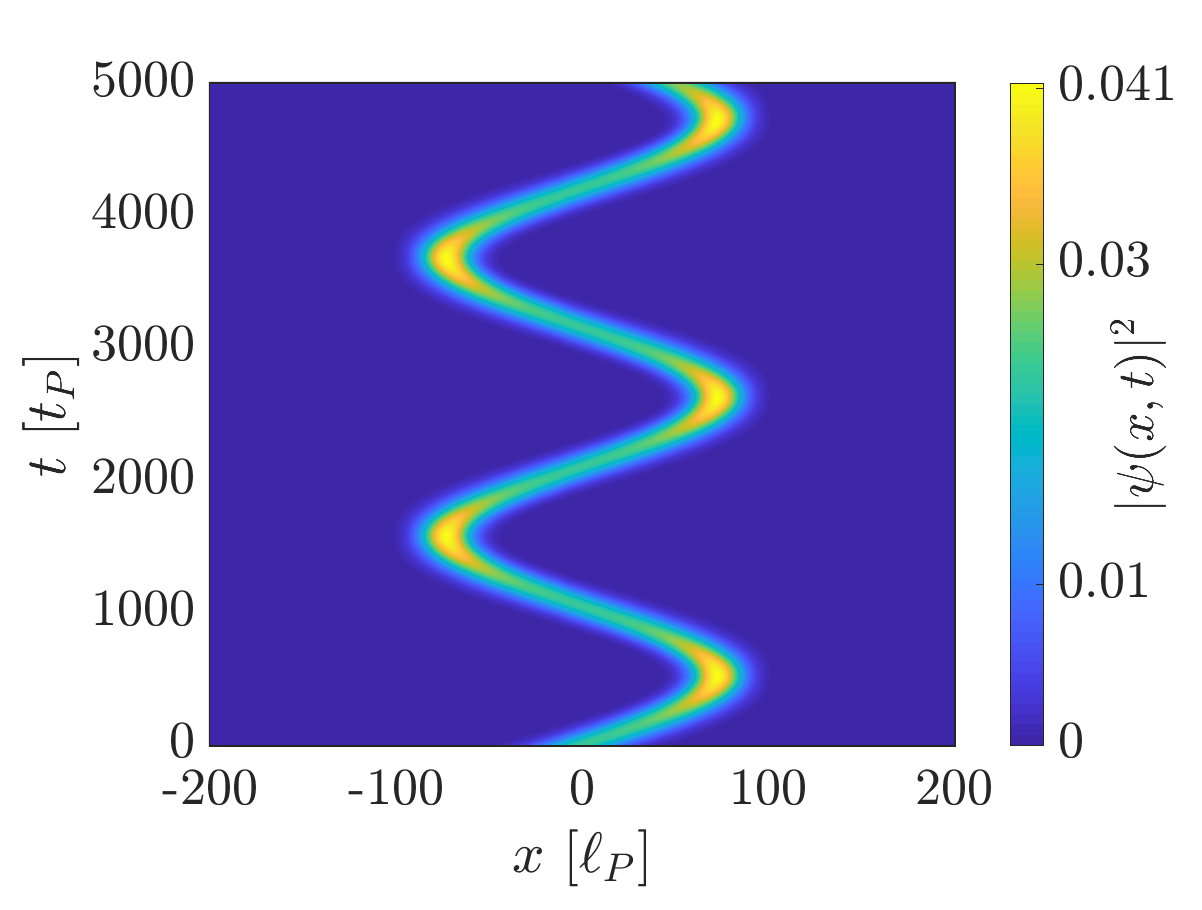
\includegraphics[width=0.5\textwidth]{graphs/i_evo.eps}
    \caption{Evolution of the system, $\Delta t = \SI{1}{\Ptime}$}
    \label{fig:i_evo}
  \end{figure}

  \subsection{Convergence studies}
    To see if the scheme works, a convergence study on multiple variables is done.
    The results are given by figure \ref{fig:i_conv}.

    \begin{figure}[h]
      \centering
      \begin{subfigure}{0.45\textwidth}
        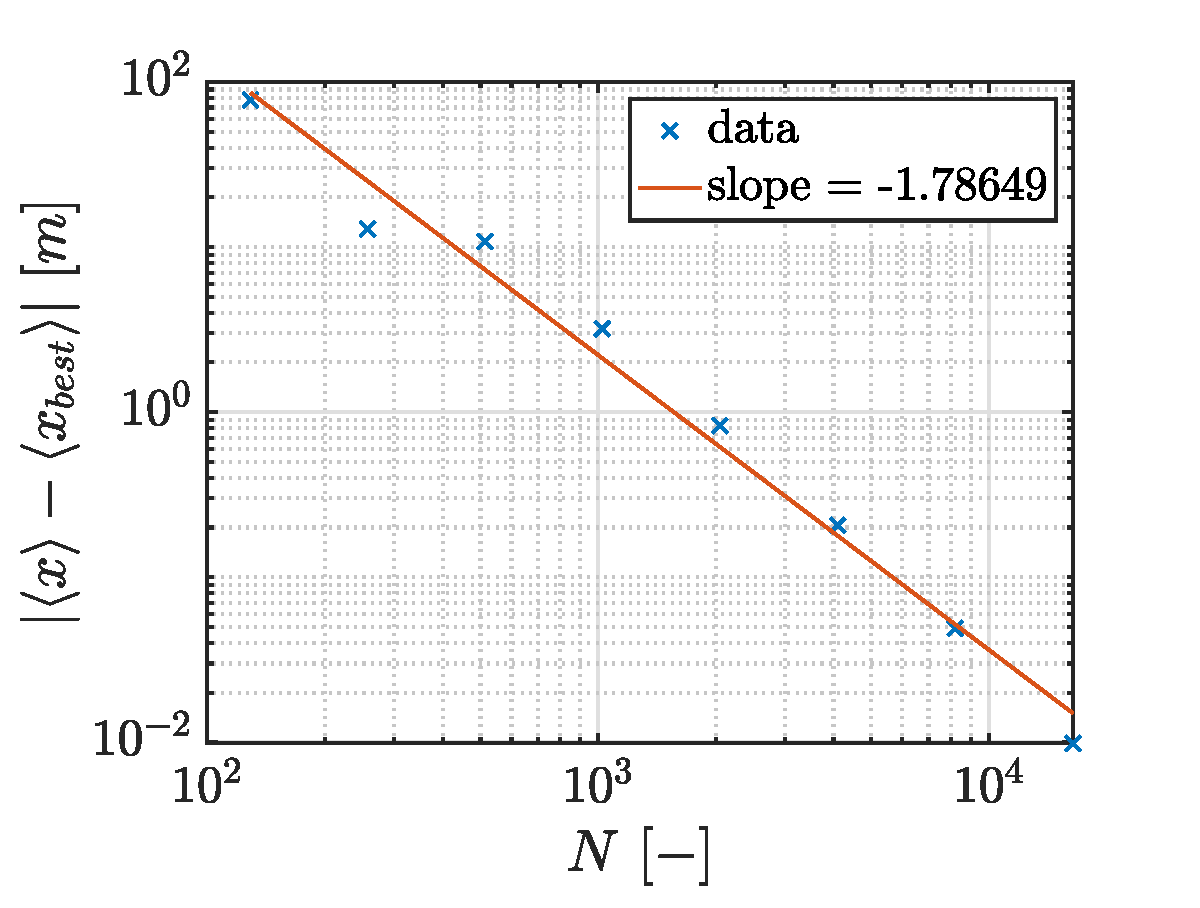
\includegraphics[width=\textwidth]{graphs/i_conv_x.eps}
        \caption{$\langle x \rangle (t)$}
        \label{fig:i_conv_x}
      \end{subfigure}
      ~
      \begin{subfigure}{0.45\textwidth}
        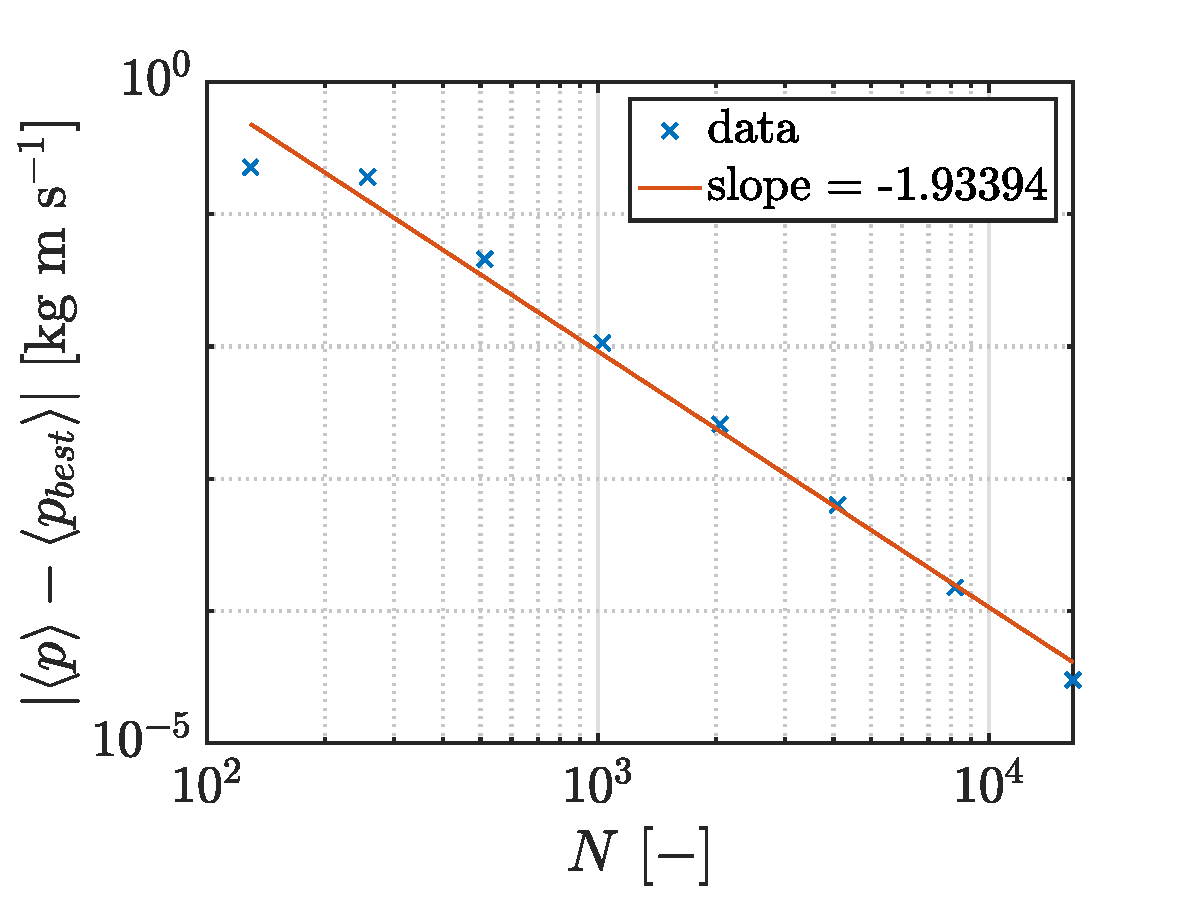
\includegraphics[width=\textwidth]{graphs/i_conv_p.eps}
        \caption{$\langle p \rangle (t)$}
        \label{fig:i_conv_p}
      \end{subfigure}
      ~
      \begin{subfigure}{0.45\textwidth}
        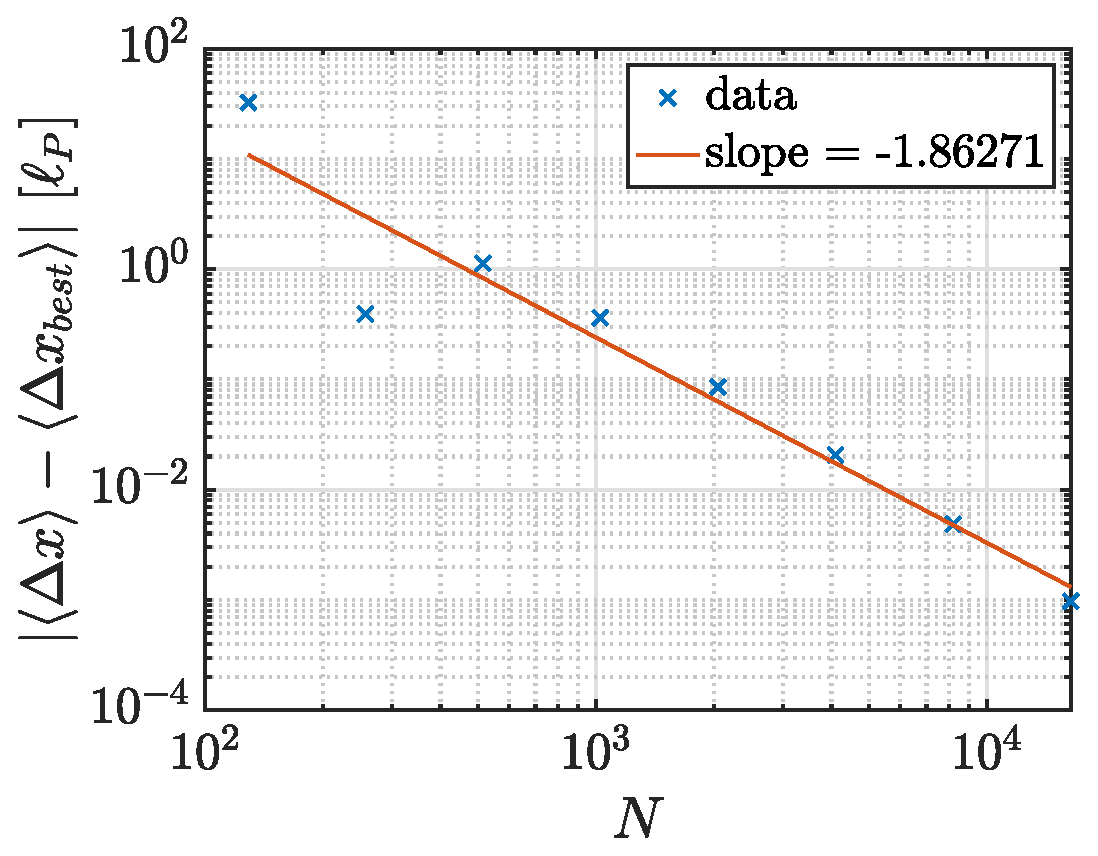
\includegraphics[width=\textwidth]{graphs/i_conv_dx.eps}
        \caption{$\langle \Delta x \rangle (t)$}
        \label{fig:i_conv_dx}
      \end{subfigure}
      ~
      \begin{subfigure}{0.45\textwidth}
        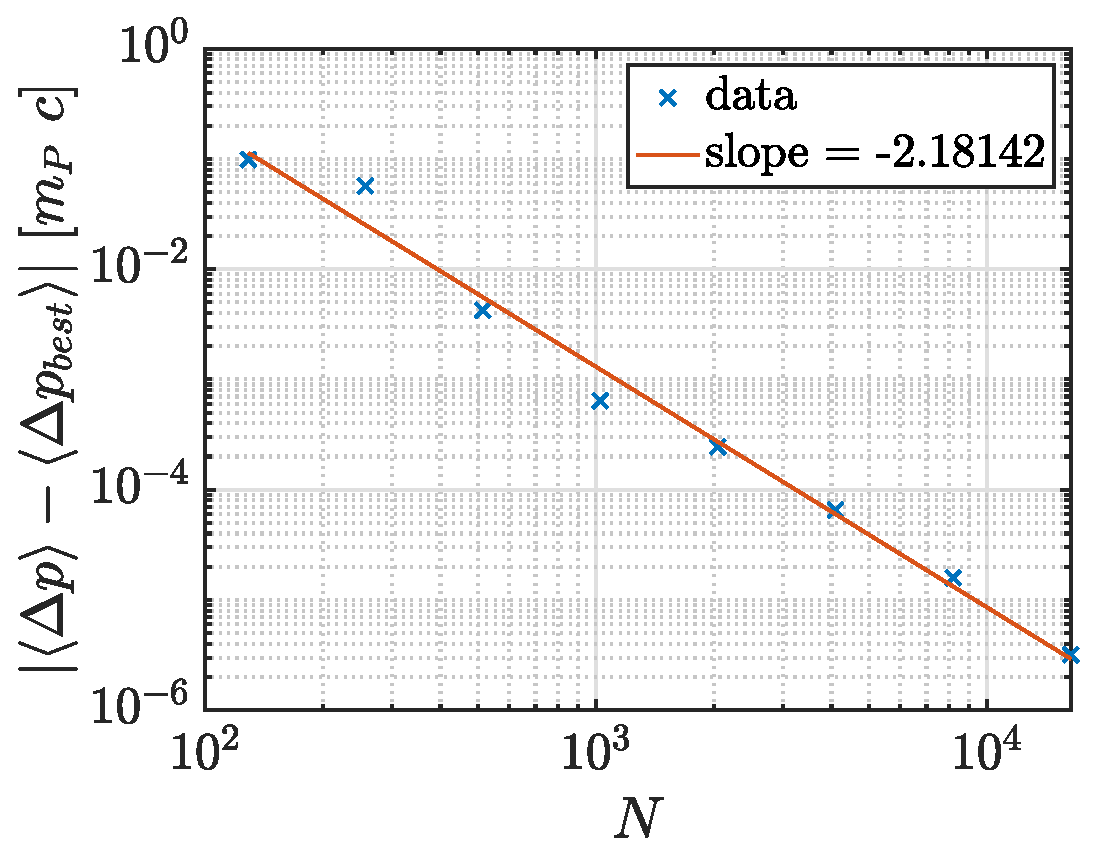
\includegraphics[width=\textwidth]{graphs/i_conv_dp.eps}
        \caption{$\langle \Delta p \rangle (t)$}
        \label{fig:i_conv_dp}
      \end{subfigure}
      \caption{Convergence study on multiple quantities with respect to $\Delta t$, with $N\in[\num{129}, \num{16380}]$ and $\Delta t = (\num{5000}/N) \si{\Ptime}$. All the values are taken at t=\SI{5000}{\Ptime}.}
      \label{fig:i_conv}
    \end{figure}

    Figure \ref{fig:i_conv} gives the convergence study on the average position $\langle x \rangle$ (Fig. \ref{fig:i_conv_x}), the average momentum $\langle p \rangle$ (Fig. \ref{fig:i_conv_p}), the average position uncertainty $\langle \Delta x \rangle$ (Fig. \ref{fig:i_conv_dx}) and the average momentum uncertainty $\langle \Delta p \rangle$ (Fig. \ref{fig:i_conv_dp}).
    These resuts show that the numerical method approximately converges on the 2nd order.
    %TODO : Je sais pas quoi dire. :|


  \subsection{Total probability}
    Next, the total probability must verify $P_\text{tot} = \Sigma_i P_i(t) = 1~\forall t$.

    Figure \ref{fig:i_ptot} gives this result, and is divided in two graphs.
    Figure \ref{fig:i_ptot_cool} gives the general behavious of both the probability on the left and the right sides of the system.
    Their sum is approximately equal to 1, and the periodicity of the system is again shown.
    Figure \ref{fig:i_ptot_ugly} gives a close look to the total probability.
    It suggests that the total probability is not exactly conserved.
    However, the vertical labels only slightly changes on a rounding error order of magnitude.
    Thus, the total probability can be considered as exactly conserved.

    \begin{figure}[h]
      \begin{subfigure}[t]{0.45\textwidth}
        \centering
        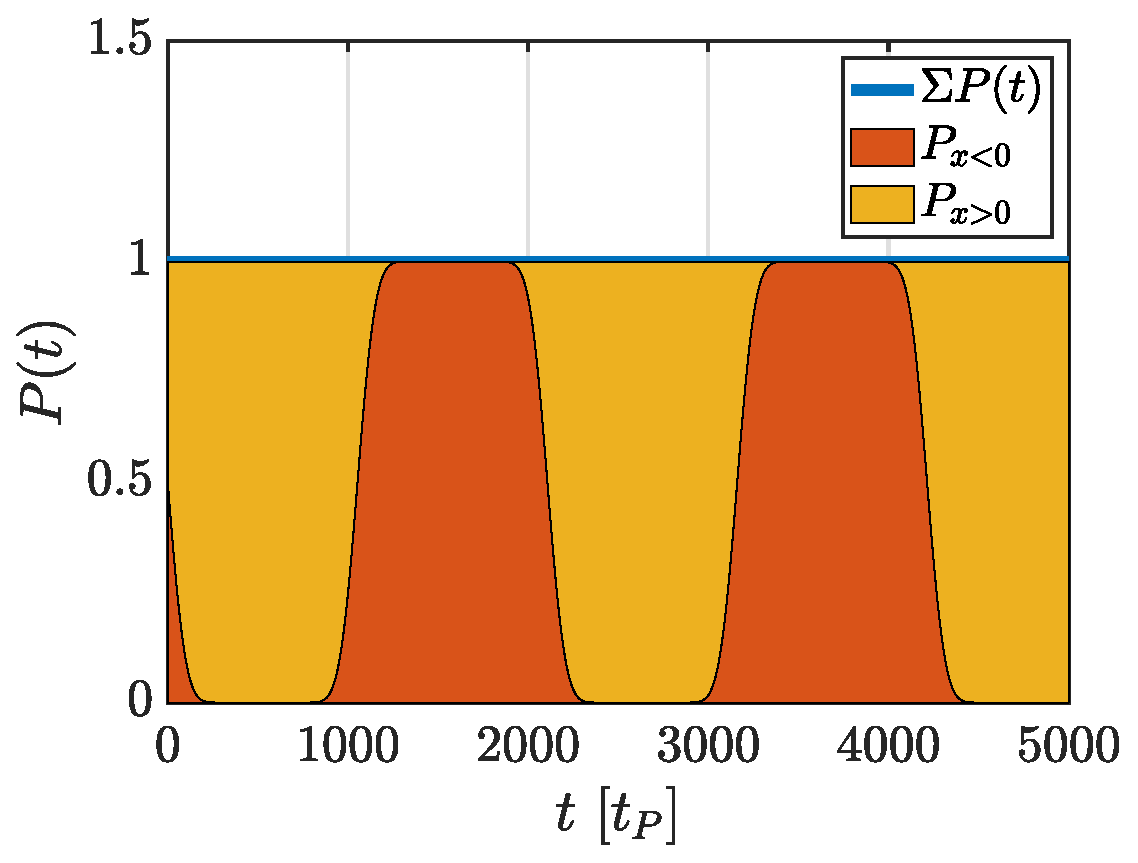
\includegraphics[width=\textwidth]{graphs/i_ptotcool.eps}
        \caption{General behavious}
        \label{fig:i_ptot_cool}
      \end{subfigure}
      ~
      \begin{subfigure}[t]{0.45\textwidth}
        \centering
        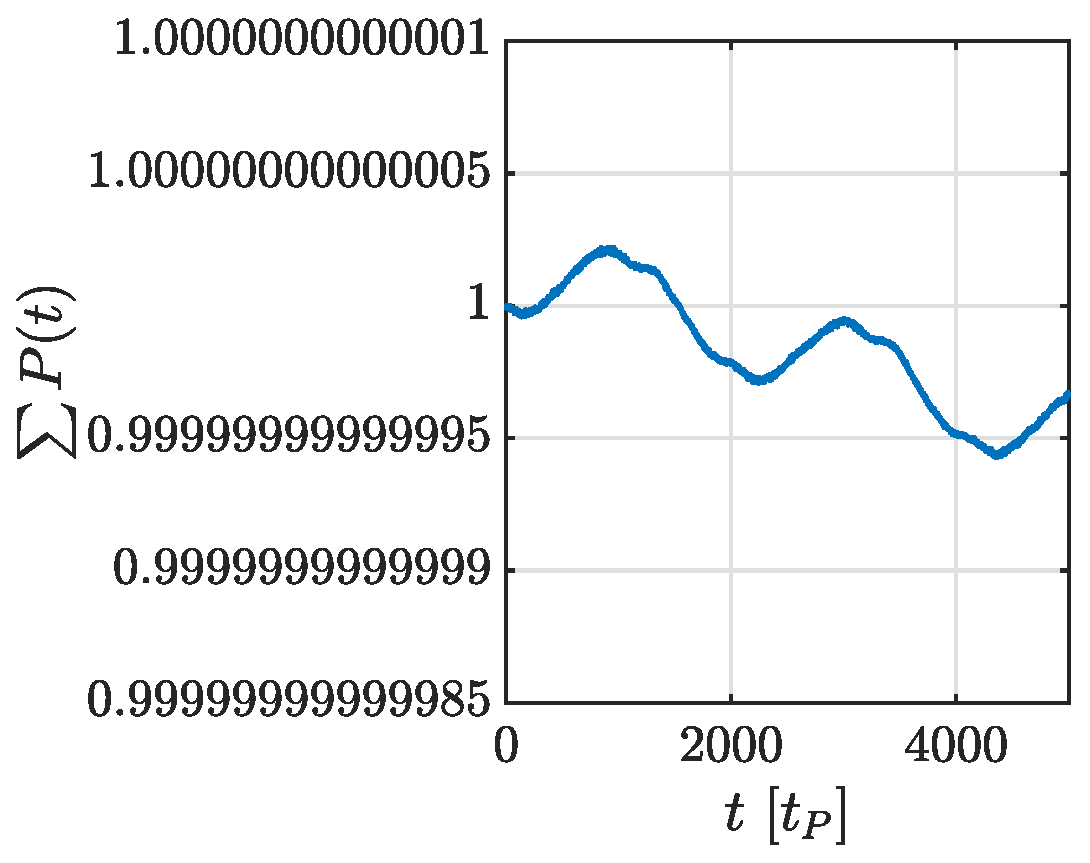
\includegraphics[width=\textwidth]{graphs/i_ptot.eps}
        \caption{Close look}
        \label{fig:i_ptot_ugly}
      \end{subfigure}
      \caption{Sum of probabilities over time, $\Delta t = \SI{1}{\Ptime}$}
      \label{fig:i_ptot}
    \end{figure}


  \subsection{Conservation of average energy}
    % Next verification is that the average energy is conserved over time.\\
    Next, the average energy must be conserved.

    Figure \ref{fig:i_E} shows that the average energy is more or less conserved.
    However, it can be observed that it slightly reduces over time, which is neglectable, as the difference is again on a rounding error order of magnitude.
    % These are the result of numerical roundings, which occures each time a value is numerically computed.
    Therefore, the average energy can be considered as exactly conserved.

    \begin{figure}[h]
      \centering
      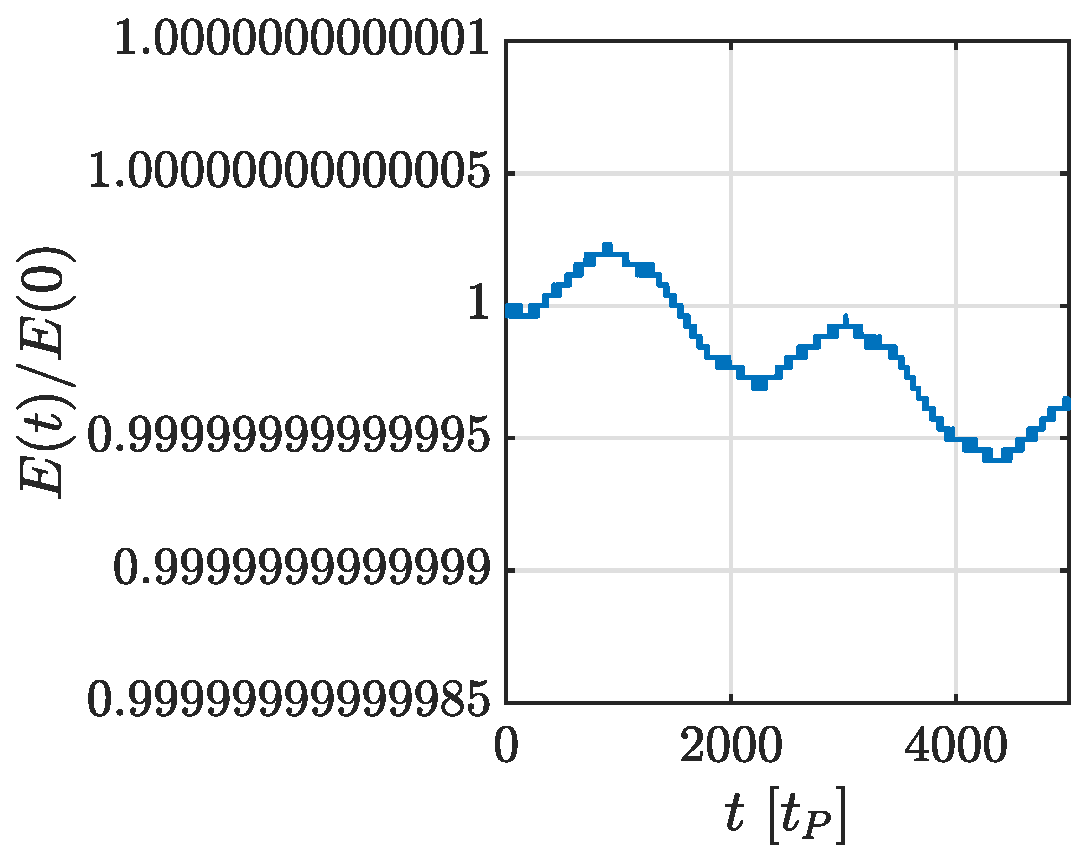
\includegraphics[width=0.45\textwidth]{graphs/i_E.eps}
      \caption{Average energy divided by the initial energy over time, $\Delta t = \SI{1}{\Ptime}$}
      \label{fig:i_E}
    \end{figure}

  \subsection{Heisenberg's uncertainty principle}
    This last part focuses on the correctness of Heisenberg's uncertainty principle, which states that $\forall t:~\langle \Delta x \rangle(t)\cdot\langle \Delta p \rangle(t) \geq \frac{\hbar}{2}$.
    Alternatively, it states that the average position and the average velocity cannot be precisely determined at the same time.
    Note that, as stated before, a normalized $\hbar$ is used, which gives $\hbar=\SI{1}{\Penergy\Ptime}$.\\

    The result is given by figure \ref{fig:i_heisenberg} and shows that the principle is overall verified.
    However, the firsts minimums of $\langle \Delta x \rangle(t)\cdot\langle \Delta p \rangle(t)$ are slightly under $\frac{\hbar}{2}$, which is explained by truncation error caused by the integral.
    But this error is vanishing over time, so it is neglectable.

    \begin{figure}[h]
      \centering
      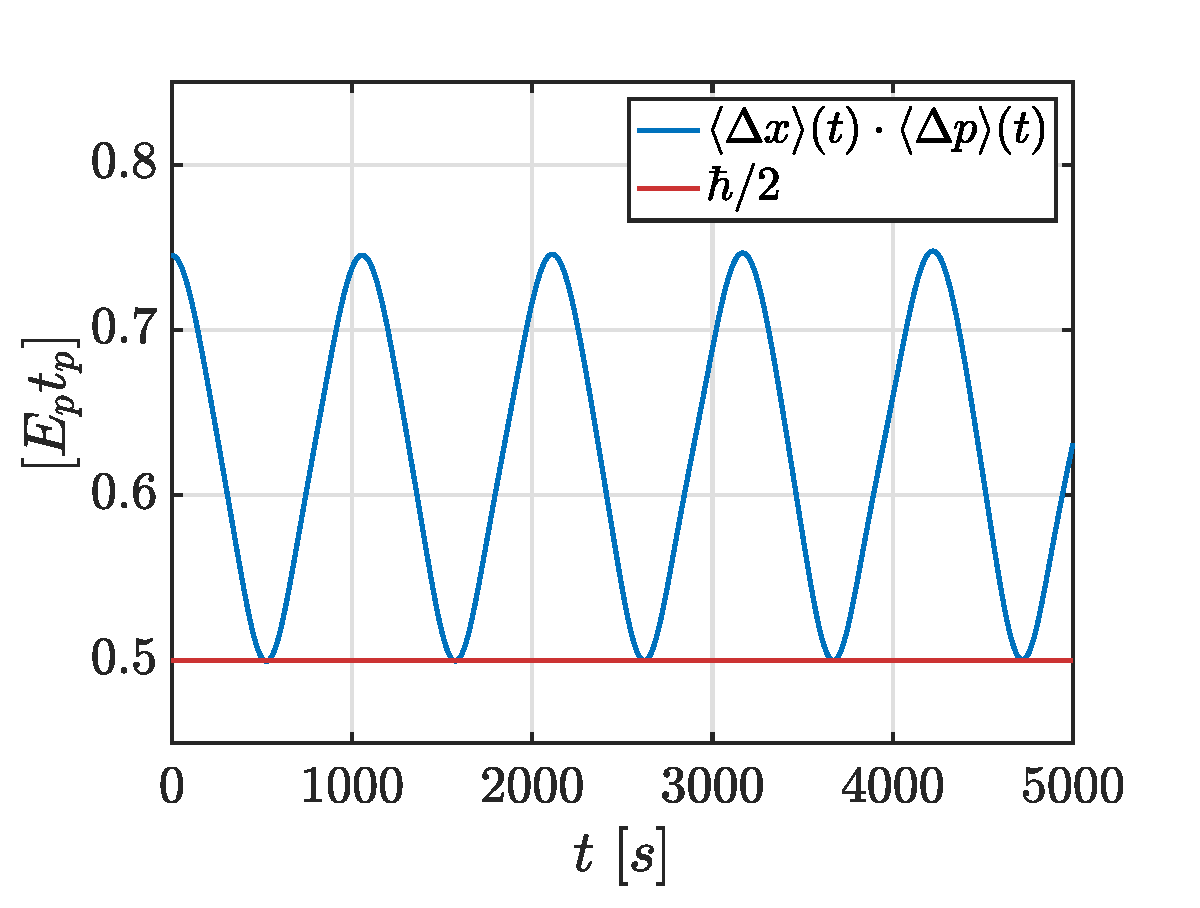
\includegraphics[width=0.45\textwidth]{graphs/i_heisenberg.eps}
      \caption{Verification of Heisenberg's principle, $\Delta t = \SI{1}{\Ptime}$}
      \label{fig:i_heisenberg}
    \end{figure}

    \subsection{Summary}
    Therefore, the conditions stated at the beginning of section \ref{sec:har_osc} describe an harmonic oscillator and the implementation from section \ref{sec:impl} works as expected.
    Further studies can thus be carried out.

%%%%%%%%%%%%%%%%%%%%%%%%%%%%%%%%%%%%%%%%%%%%%%%%%%

\newpage
\section{Average movement analysis for a particle and comparison with the classical case}

With the same parameters as in section \ref{sec:har_osc}, the average position and momentum of the particle is analysed and compared to the analytical solution, which is found using the Ansatz for a harmonic oscillator with potential $V(x)=\frac{1}{2}m\omega^2x^2$:
\begin{equation}
 x(t)=A \cos(\omega t) + B \sin(\omega t)
 \label{eq:ansatz}
\end{equation}
where $A$ and $B$ are constants found with the initial conditions: since $x(0)=x_0$, we have $A=x_0$, and from $\dot{x}(t)=p_0/m$ and $p_0=\hbar k_0$, by taking the derivative of eq. \eqref{eq:ansatz}, we get $B=\hbar k_0/m\omega$. The solution is thus:
\begin{align}
 &x(t)=x_0\cos(\omega t) + \frac{\hbar k_0}{m \omega} \sin(\omega t)\\
 &p(t)=m\dot{x}(t)=-m\omega x_0\sin(\omega t) + \hbar k_0 \cos(\omega t)
\end{align}
Here, $x_0=0$, $m=1$ and $\hbar=1$. The results of these comparisons are displayed in figure \ref{fig:ii}.


\begin{figure}[h!]
\begin{subfigure}[t]{0.46\textwidth}
 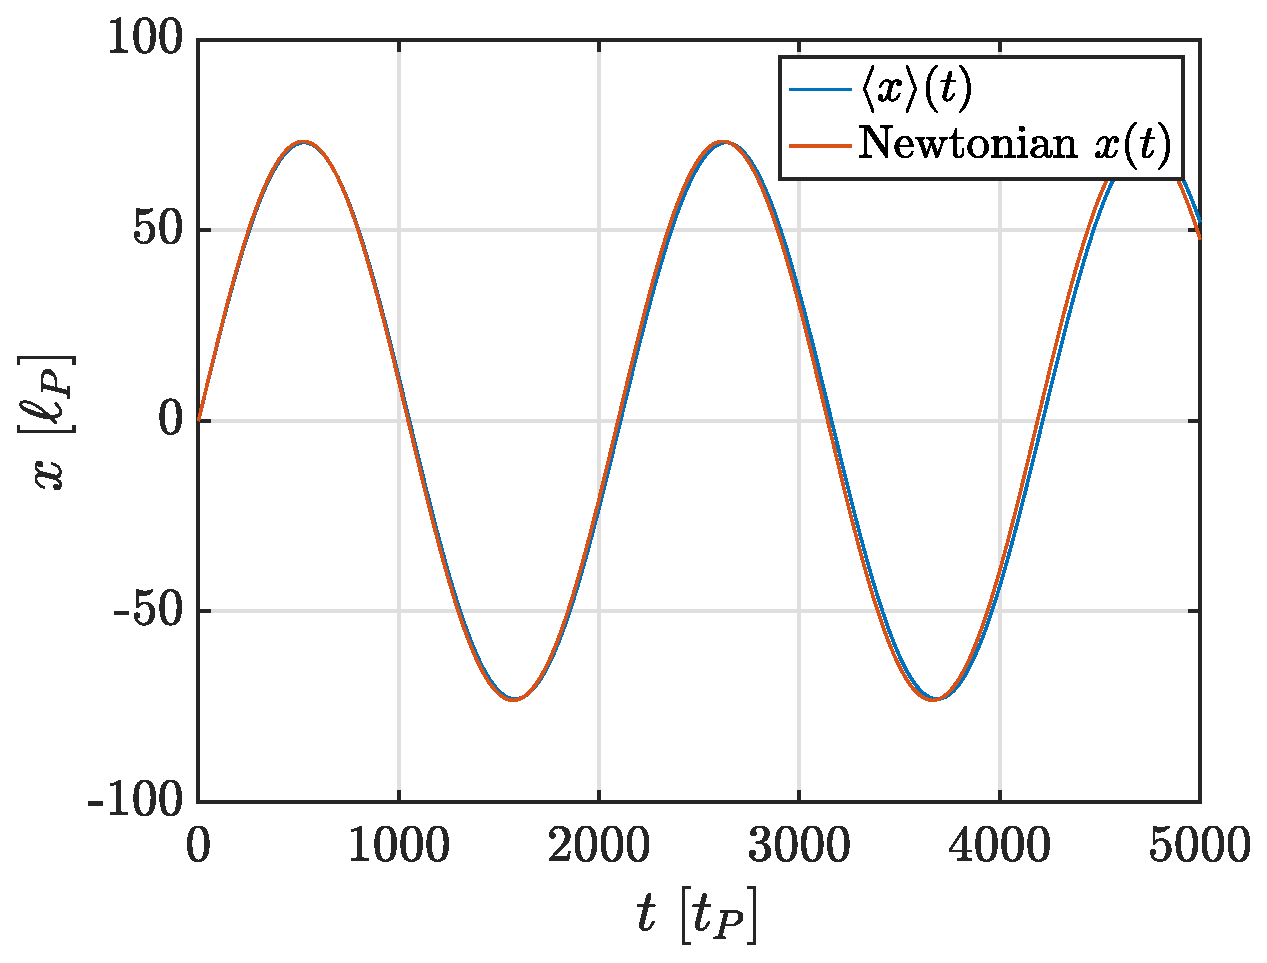
\includegraphics[width=\textwidth]{graphs/ii_x.eps}
 \caption{Particle movement}
\end{subfigure}
~
\begin{subfigure}[t]{0.46\textwidth}
 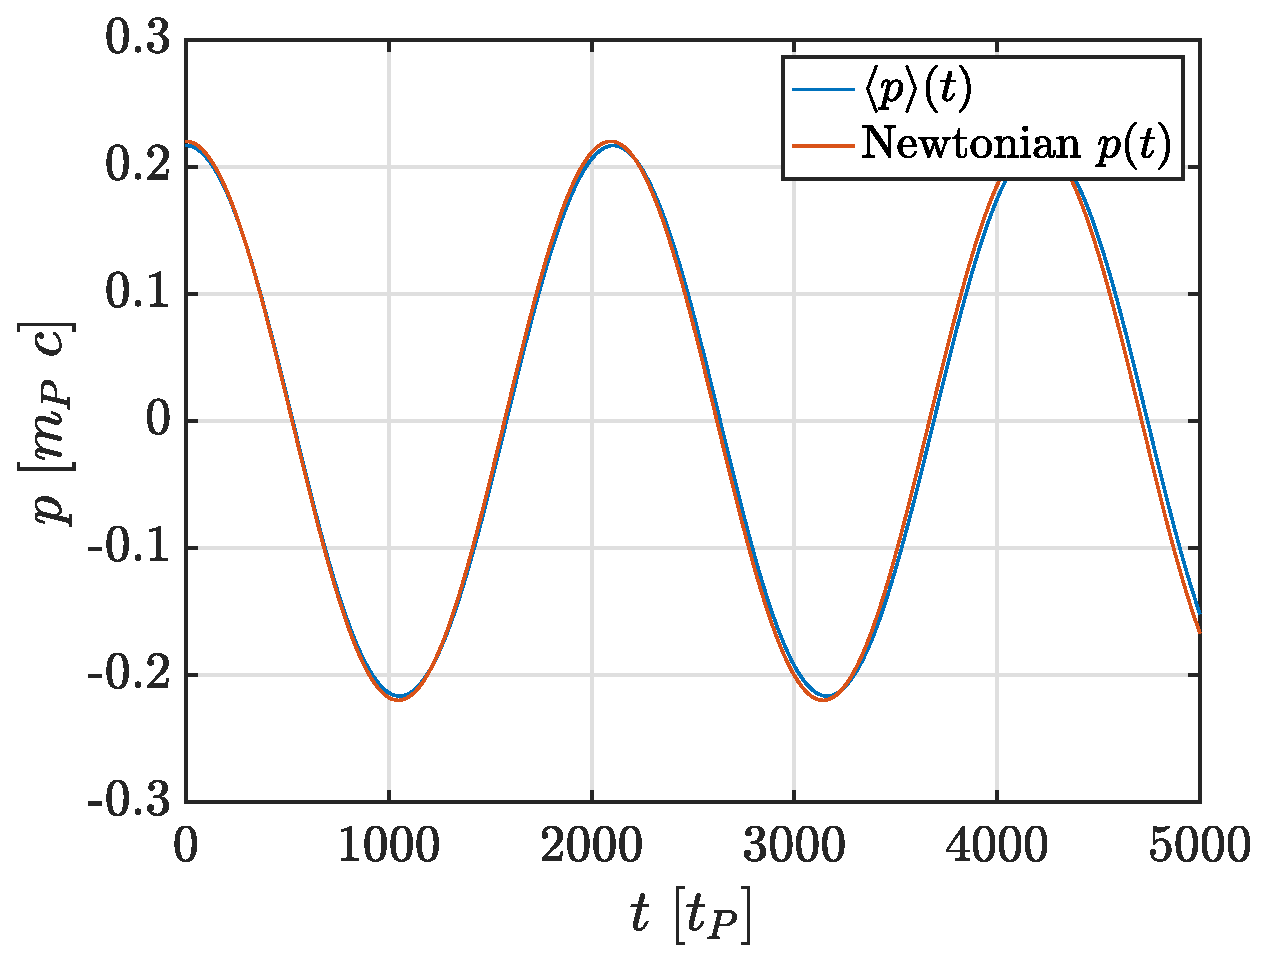
\includegraphics[width=\textwidth]{graphs/ii_p.eps}
 \caption{Particle momentum}
\end{subfigure}
\caption{Comparison of the simulated position and momentum of the particle with their respective classical analytical solutions}
\label{fig:ii}
\end{figure}

The general behavior for both the average position and the average momentum of the particle is that of a harmonic oscillator. For these parameters, the simulations follow the classical solution quite closely. $\langle x \rangle (t)$ and $x(t)$ both start out at 0 at $t=0$, while $\langle p \rangle (t)$ and $p(t)$ start out with a small difference at $t=0$. A more detailed analysis of the differences between the simulations and the classical solutions is displayed on figures \ref{fig:ii_diffx} and \ref{fig:ii_diffp}.

\begin{figure}[h!]
 \begin{subfigure}[t]{0.45\textwidth}
 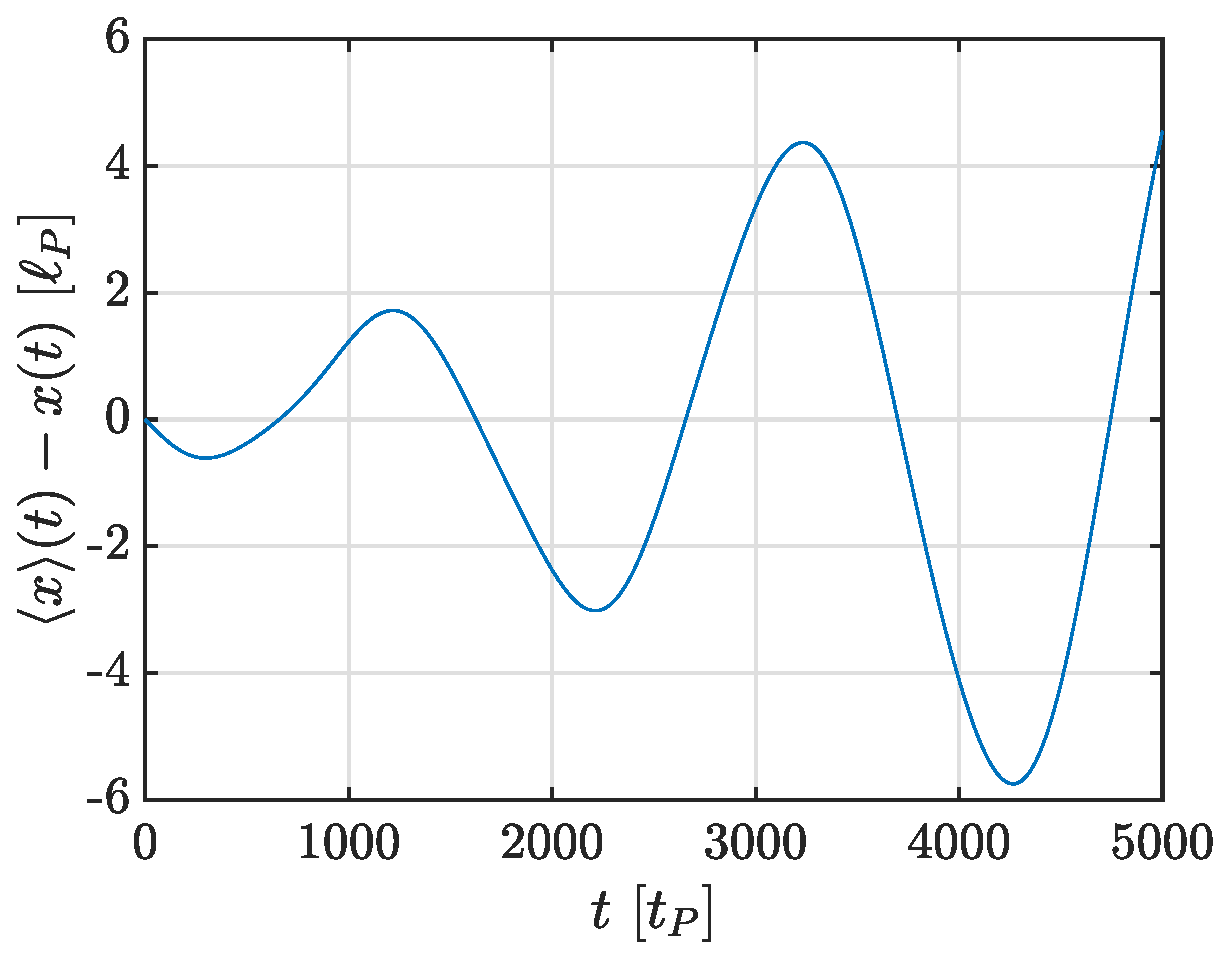
\includegraphics[width=\textwidth]{graphs/ii_diffx.eps}
  \caption{Difference over the total time of the simulation}
 \end{subfigure}
 ~
 \begin{subfigure}[t]{0.45\textwidth}
 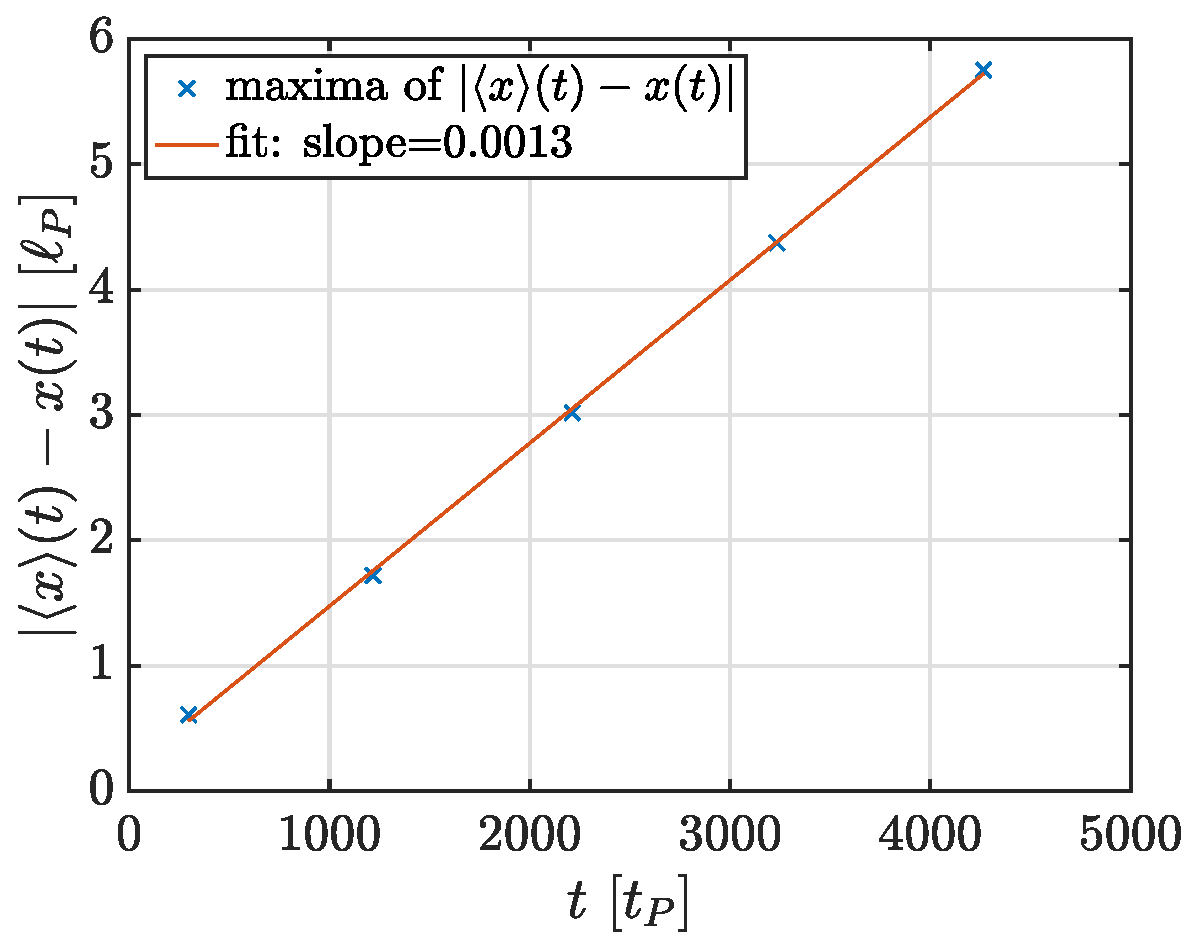
\includegraphics[width=\textwidth]{graphs/ii_diffxsl.eps}
  \caption{Maxima of the absolute difference}
 \end{subfigure}
\caption{Evolution of the difference between the simulated position and its classical solution}
\label{fig:ii_diffx}
\end{figure}

\begin{figure}[h!]
 \begin{subfigure}[t]{0.45\textwidth}
 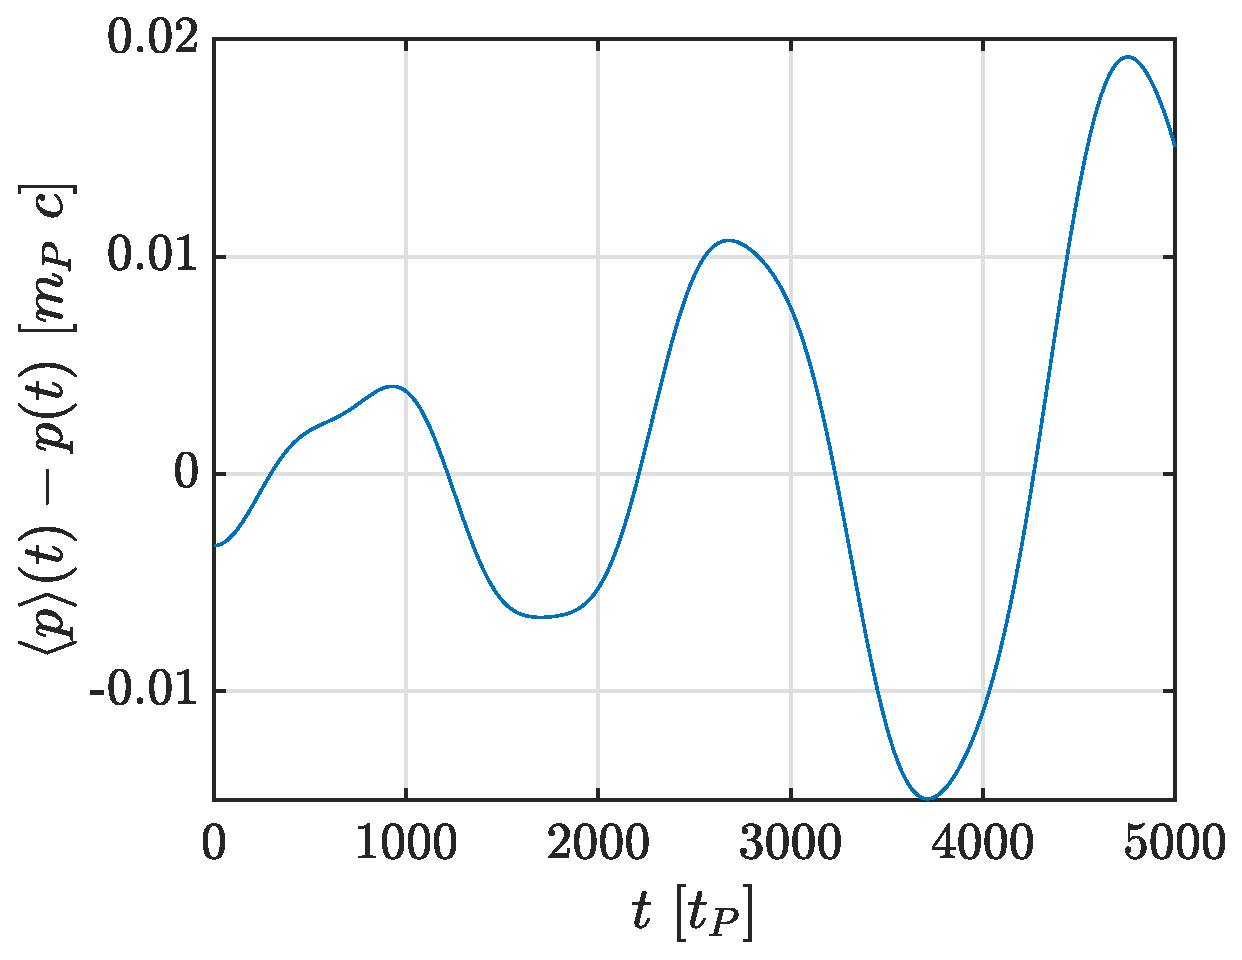
\includegraphics[width=\textwidth]{graphs/ii_diffp.eps}
  \caption{Difference over the total time of the simulation}
 \end{subfigure}
 ~
 \begin{subfigure}[t]{0.45\textwidth}
 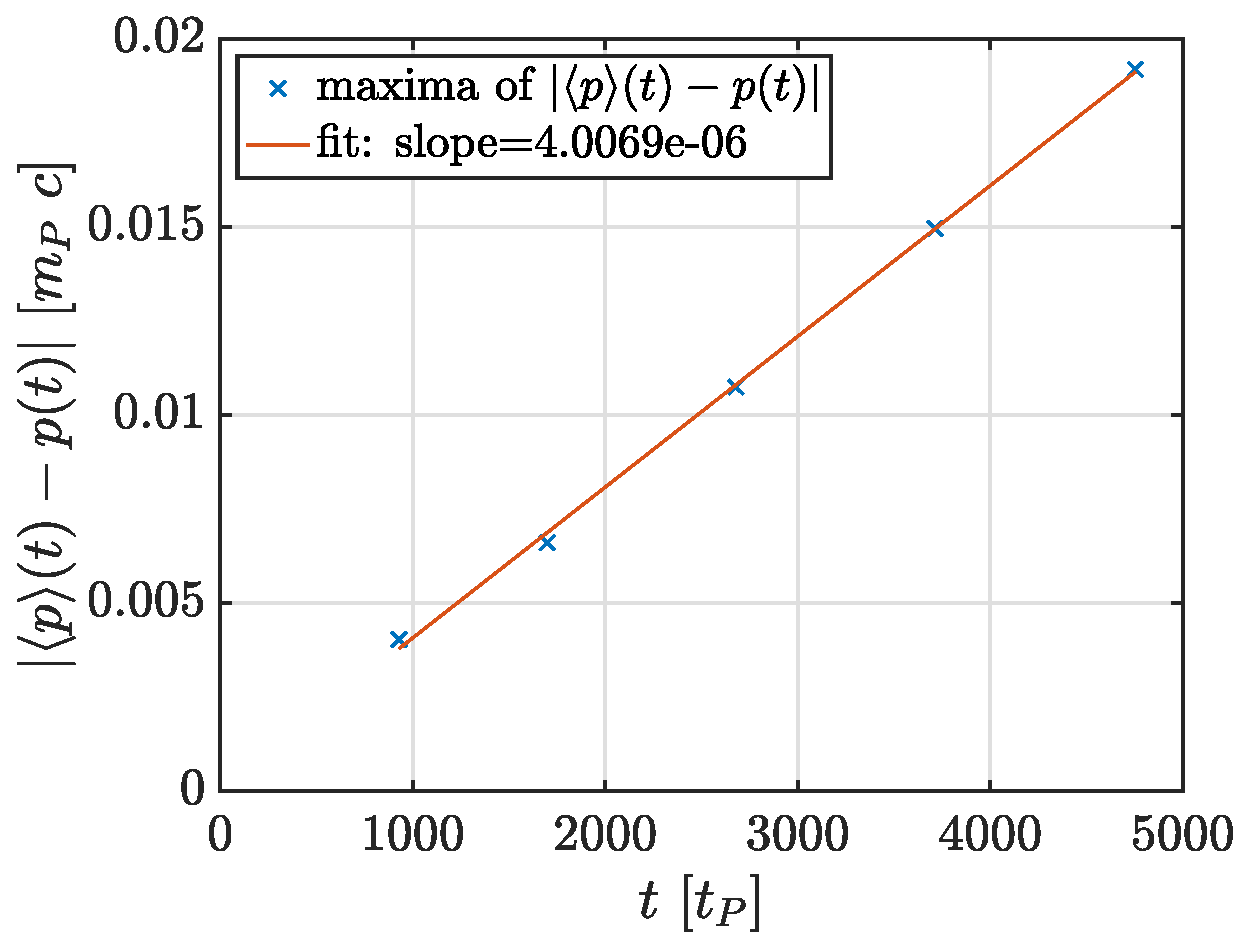
\includegraphics[width=\textwidth]{graphs/ii_diffpsl.eps}
 \caption{Maxima of the absolute difference}
 \end{subfigure}
\caption{Evolution of the difference between the simulated momentum and its classical solution}
\label{fig:ii_diffp}
\end{figure}

In both cases the difference oscillates around zero with linearly increasing amplitude. The oscillations for the difference on the position seem quite regular, while the curve for the difference on the momentum is more misshapen. Moreover the rate of the increase in amplitude of the oscillations for the difference on the position is around 3 orders of magnitude higher than that of the momentum.

%%%%%%%%%%%%%%%%%%%%%%%%%%%%%%%%%%%%%%%%%%%%%%%%%%

\newpage
\section{Quantum tunnelling}\label{sec:quantum_tunnelling}
  Quantum tunnelling is an effect of quantum physics where particles overcome potential barriers. \cite{wiki:quantum_tunnelling}
  This section will thus focus on the study of this effect by means of the implementation described in section \ref{sec:impl}.\\

  \subsection{Emphasis of quantum tunnelling}
    To emphasis this effect, the height of the potential barrier $V_0 = V(x=0)$ will be changed to three different values: $V_0<E$, $V_0 \approx E$ and $V_0>E$.
    This barrier can be change using $\Delta$ and $x_0 = -\Delta$.
    The other parameters for this section are given by $x_L=\SI{-200}{\Plength}$, $x_R=\SI{200}{\Plength}$, $\omega = \SI{0.003}{\Pangularfrequency}$, $\sigma_\text{norm} = \SI{0.06}{\Plength}$, $n=14$, $t_\text{fin} = \SI{5000}{\Ptime}$, $N_\text{inters} = 300$ and $\Delta t = \SI{2}{\Ptime}$.\\

    Figure \ref{fig:iii_evo_Egeqv0} gives the evolution of the system when $E > V_0$.
    As the potential barrier is smaller than the total energy, the particle freely flows from one side to the other, as shows by figure \ref{fig:iii_evo_Egeqv0_evo}.
    Figure \ref{fig:iii_evo_Egeqv0_prob} shows that the probability for the particle to be each side is periodically inverted, which again shows that the barrier potential is not a problem in this case.
    No quantum tunnelling takes place here.\\

    \begin{figure}[h]
      \centering
      \begin{subfigure}[t]{0.45\textwidth}
        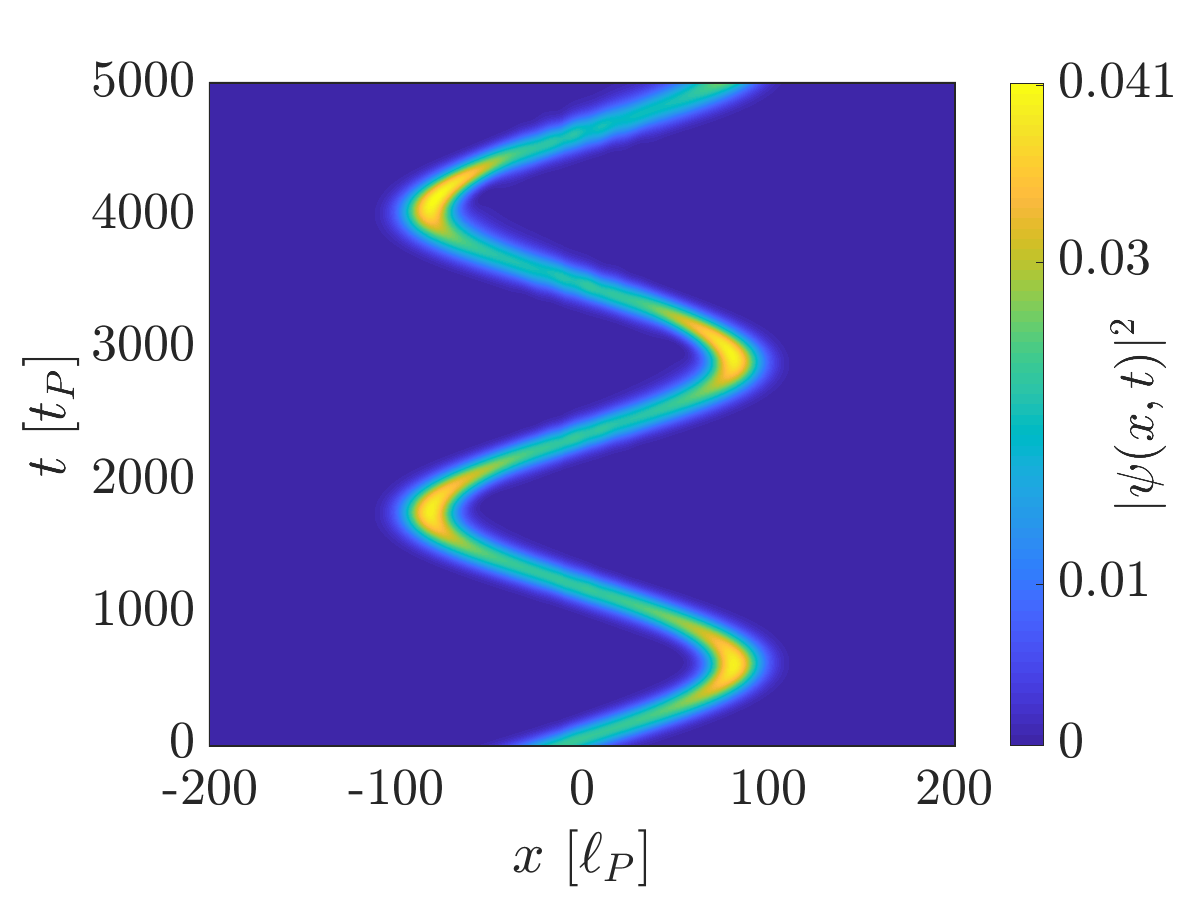
\includegraphics[width=\textwidth]{graphs/iii_evo_Egeqv0_evo.eps}
        \caption{$|\psi(x, t)|^2$ with respect to $x$ and t}
        \label{fig:iii_evo_Egeqv0_evo}
      \end{subfigure}
      ~
      \begin{subfigure}[t]{0.45\textwidth}
        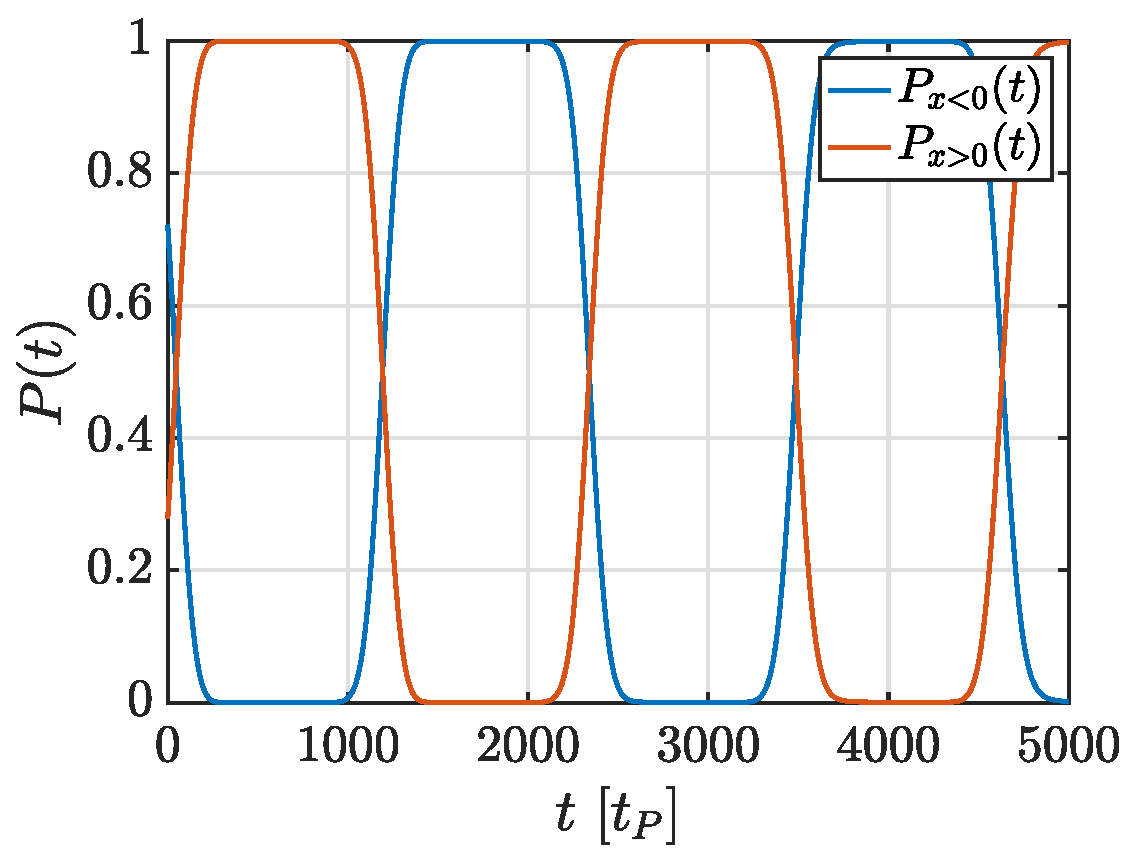
\includegraphics[width=\textwidth]{graphs/iii_evo_Egeqv0_prob.eps}
        \caption{$P(t)$ with respect to t}
        \label{fig:iii_evo_Egeqv0_prob}
      \end{subfigure}
      \caption{Evolution of the particle for $\Delta = \SI{10}{\Plength}$, which gives $E > V_0$}
      \label{fig:iii_evo_Egeqv0}
    \end{figure}

    Figure \ref{fig:iii_evo_Eeqv0} gives the evolution of the system when $E \approx V_0$.
    This time, the particle should not be able to overcome the potential barrier without taking the quantum tunnelling into account.
    What can be observed on figure \ref{fig:iii_evo_Eeqv0_evo} is the fact that the particle still has a probability to reach the other side of the potentiel barrier.
    Figure \ref{fig:iii_evo_Eeqv0_prob} strengthens this observation.
    This is a great evidence of quantum tunnelling, as it is the only explaination why particles have a probability of overcoming the potential barrier.\\


    \begin{figure}[h]
      \centering
      \begin{subfigure}[t]{0.45\textwidth}
        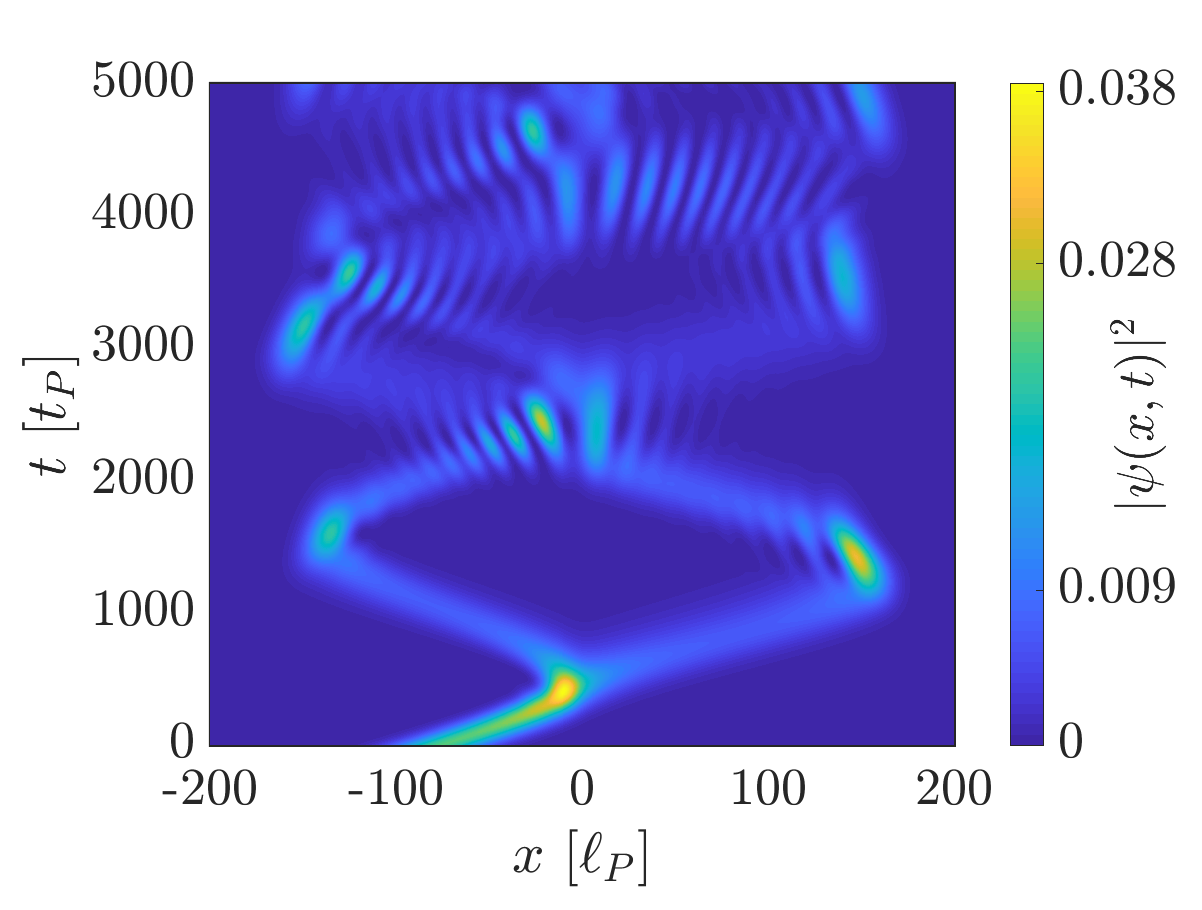
\includegraphics[width=\textwidth]{graphs/iii_evo_Eeqv0_evo.eps}
        \caption{$|\psi(x, t)|^2$ with respect to $x$ and t}
        \label{fig:iii_evo_Eeqv0_evo}
      \end{subfigure}
      ~
      \begin{subfigure}[t]{0.45\textwidth}
        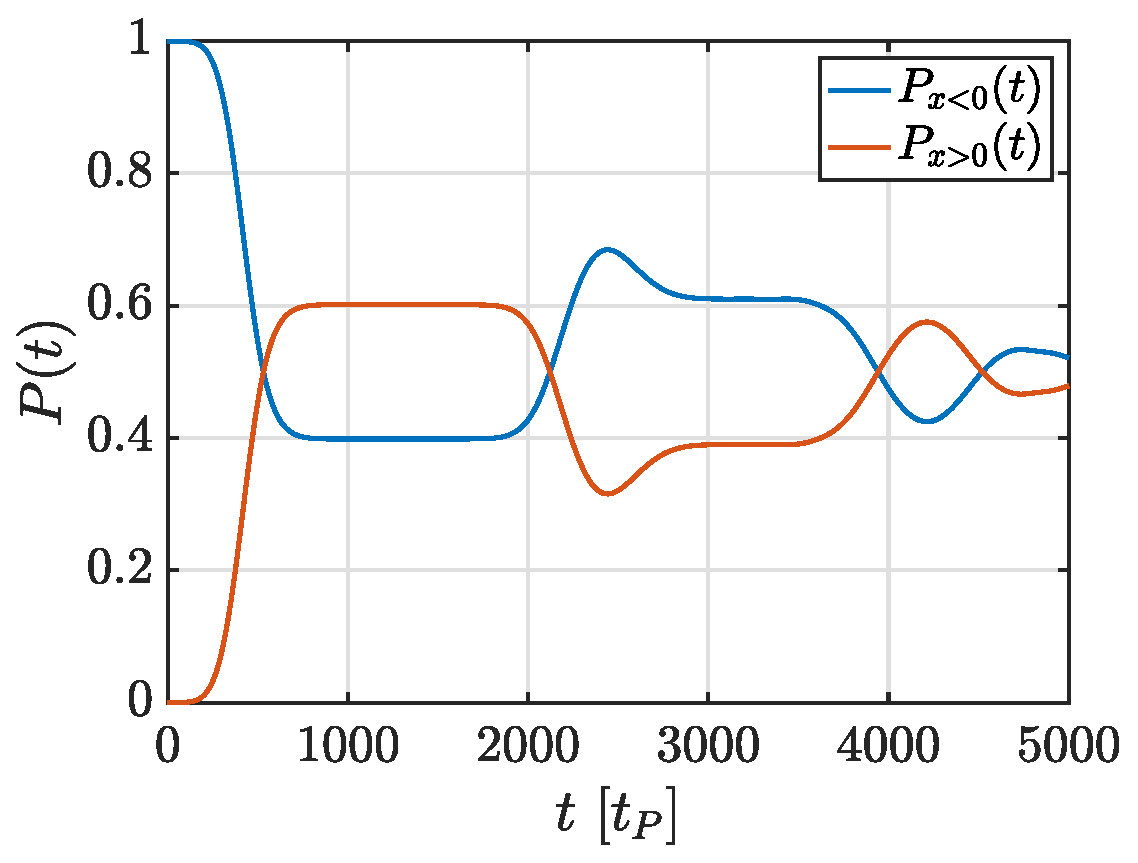
\includegraphics[width=\textwidth]{graphs/iii_evo_Eeqv0_prob.eps}
        \caption{$P(t)$ with respect to t}
        \label{fig:iii_evo_Eeqv0_prob}
      \end{subfigure}
      \caption{Evolution of the particle for $\Delta \approx \SI{75.57}{\Plength}$, which gives $E \approx V_0$}
      \label{fig:iii_evo_Eeqv0}
    \end{figure}

    Finally, figure \ref{fig:iii_evo_Eleqv0} gives the evolution of the system when $E<V_0$.
    This time, the potential barrier is to high compared to the energy, which results with a particle stuck in a side with no probability of being on the other side.
    Figures \ref{fig:iii_evo_Eleqv0_evo} and \ref{fig:iii_evo_Eleqv0_prob} shows this fact, as the probability for the particle to be on the right side is approximately null.\\

    \begin{figure}[h]
      \centering
      \begin{subfigure}[t]{0.45\textwidth}
        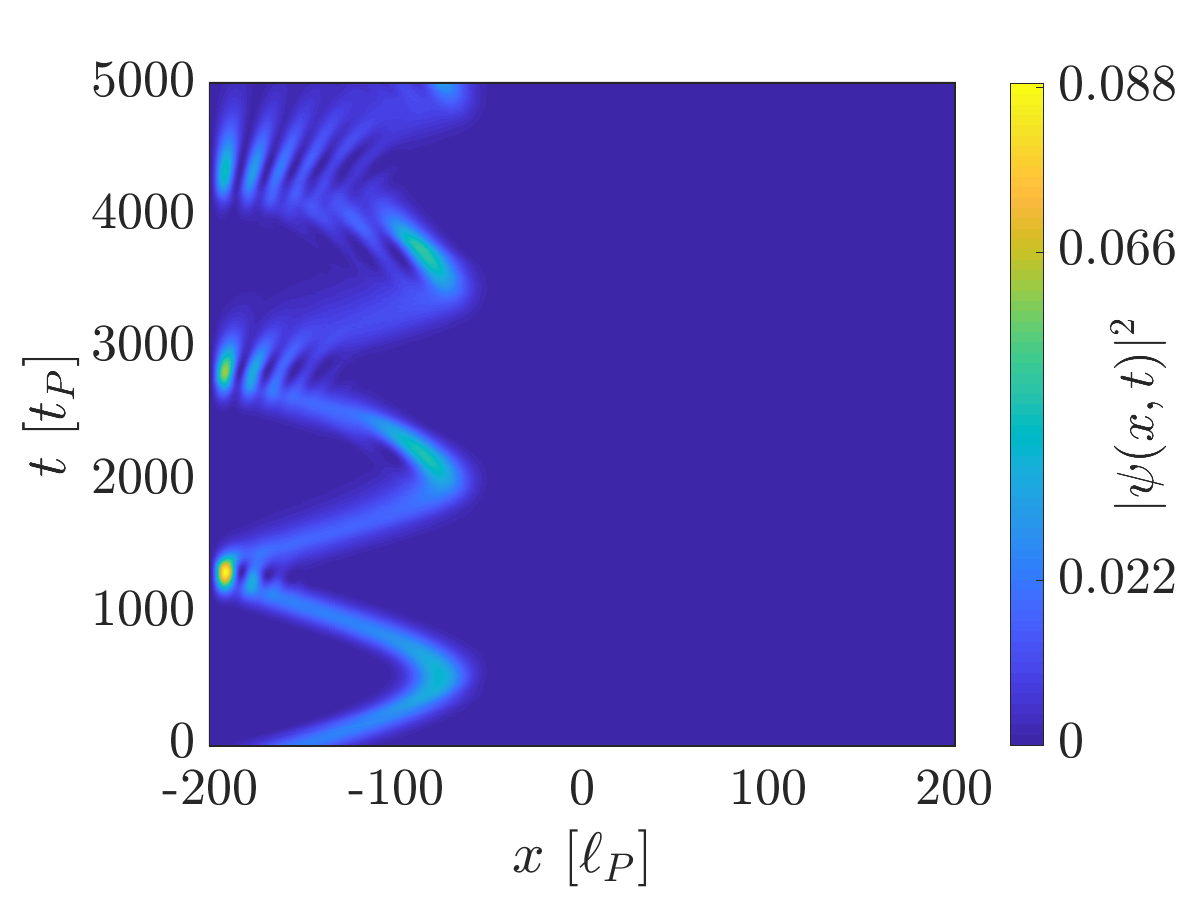
\includegraphics[width=\textwidth]{graphs/iii_evo_Eleqv0_evo.eps}
        \caption{$|\psi(x, t)|^2$ with respect to $x$ and t}
        \label{fig:iii_evo_Eleqv0_evo}
      \end{subfigure}
      ~
      \begin{subfigure}[t]{0.45\textwidth}
        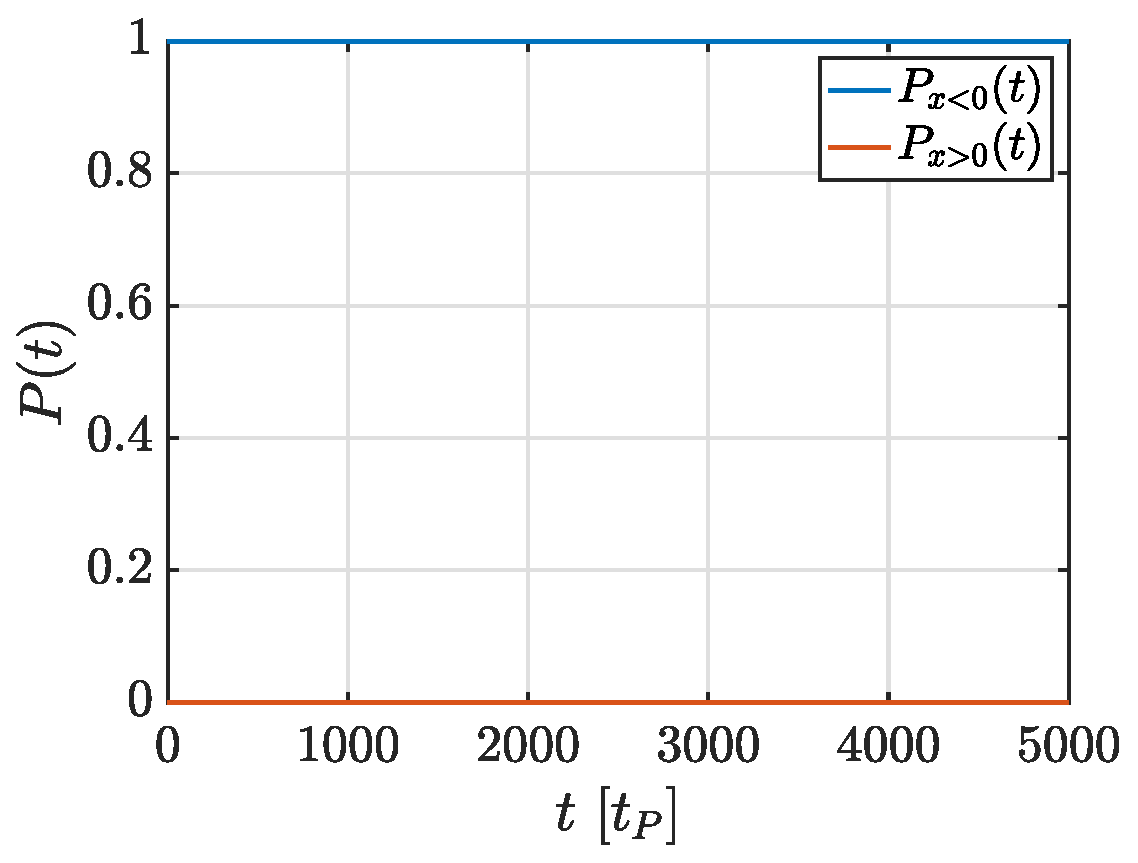
\includegraphics[width=\textwidth]{graphs/iii_evo_Eleqv0_prob.eps}
        \caption{$P(t)$ with respect to t}
        \label{fig:iii_evo_Eleqv0_prob}
      \end{subfigure}
      \caption{Evolution of the particle for $\Delta = \SI{150}{\Plength}$, which gives $E < V_0$}
      \label{fig:iii_evo_Eleqv0}
    \end{figure}

    Thus, this section has shown that quantum tunnelling is a notable effect of quantum physics and much be taken into account when the potential barrier is around the total energy.
    However, when the potential barrier is \textit{significantly} higher than the total energy, this effect becomes neglectable.\\

  \subsection{\SI{50}{\percent} tunnelling probability}
    This second section focuses on finding the right value for $n$ that gives a tunnelling probability of \SI{50}{\percent} for $\Delta = \SI{64}{\Plength}$.
    To obtain this value, the difference of probabilities between both side at \SI{1000}{\Ptime} (when the probability in both sides are clearly separated) has been plotted with respect to $n$.
    This gives the values $n$ where the probability on both sides are the closest, which is \SI{50}{\percent}.
    The parameter $n$ is initially an integer used to define the wavenumber, which is given by $k_0 = 2\pi n/(x_R-x_L)$.
    However, the best result is still far from an exact \SI{50}{\percent}, so the implementation has been modified to allow a real $n$.
    Both version are analysed in the following sections.\\

    \subsubsection{$n$ as an integer}
      First, $n$ is considered as an integer.
      Figure \ref{fig:iii_findn_n} shows the study of the difference of probabilities with respect to $n$.
      The value the closest to a \SI{50}{\percent} tunnelling probability is given by $n = 11$, with a difference of $\abs{P_{x<0} - P_{x>0}} \approx \SI{2.1}{\percent}$.\\

      \begin{figure}[h]
        \centering
        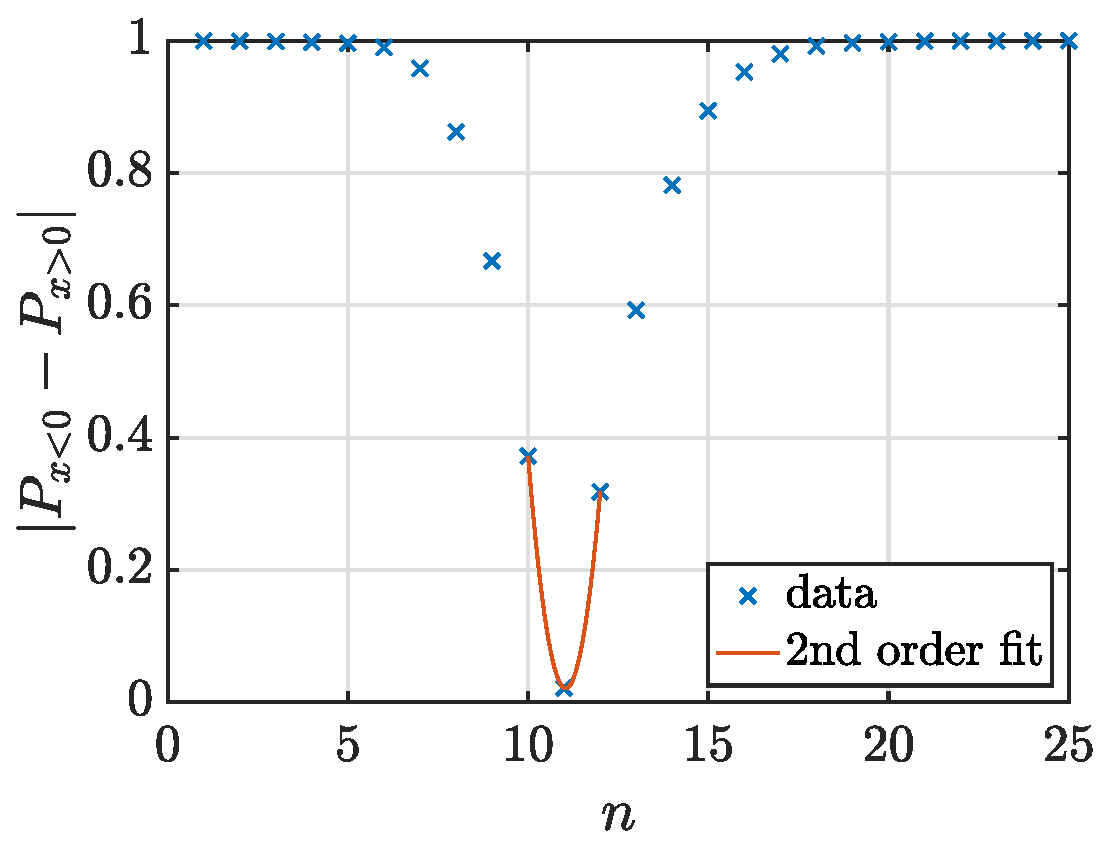
\includegraphics[width=0.45\textwidth]{graphs/iii_findn_n_approx.eps}
        \caption{Difference of probabilities with respect to integer n for $\Delta = \SI{64}{\Plength}$ and $\Delta t = \SI{5}{\Ptime}$, with a 2nd order fit for the best values}
        \label{fig:iii_findn_n}
      \end{figure}

      The evolution of the system with $n=11$ is given by figure \ref{fig:iii_findn}.
      Figure \ref{fig:iii_findn_evo} gives the evolution of the density of probability $\abs{\psi(x,t)}^2$ over time and space.
      It shows that the particle has almost the same probability of being on both sides.
      This result is reinforced by figure \ref{fig:iii_findn_prob}, which shows the evolution of probability over time.
      It can be seen that around $\SI{1000}{\Ptime}$, which is the beginning of the first stable section, the probability of being on each side is approximately the same, as expected.\\

      However, this result is limited by the fact that $n$ is integer.
      To improve the result, an interpolation by a second order curve of the three best $n$ is done, as shown on figure \ref{fig:iii_findn_n}.
      This way, a more accurate value of $n$, based on the current result can be approximated, and is given by $n\approx\num{11.04}$.
      To further improve this result, it is also possible to change the implementation, and consider $n$ as a real number.
      Thus, the next section will apply the same study to a real $n$, in order to improve the result.\\

      \begin{figure}[h]
        \centering
        \begin{subfigure}[t]{0.45\textwidth}
          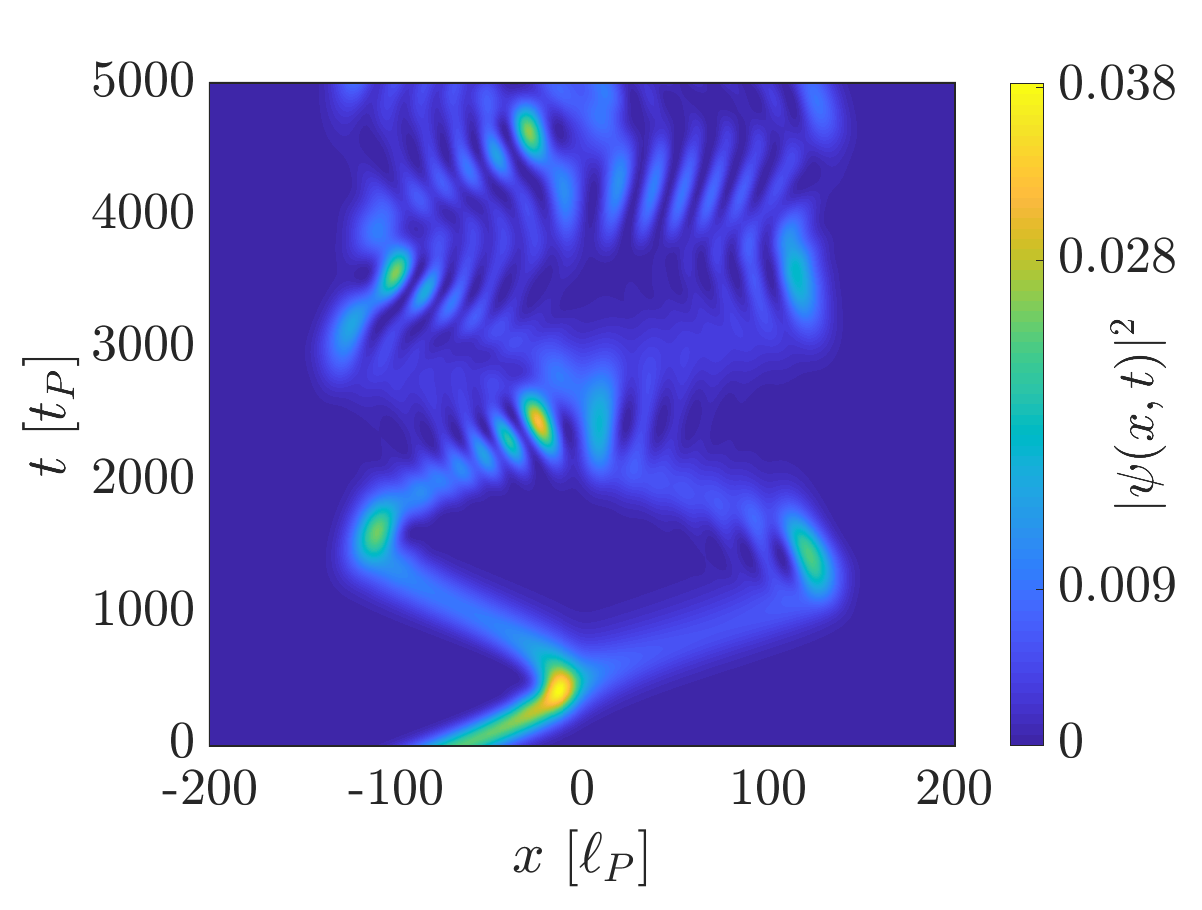
\includegraphics[width=\textwidth]{graphs/iii_findn_evo.eps}
          \caption{$|\psi(x, t)|^2$ with respect to $x$ and t}
          \label{fig:iii_findn_evo}
        \end{subfigure}
        ~
        \begin{subfigure}[t]{0.45\textwidth}
          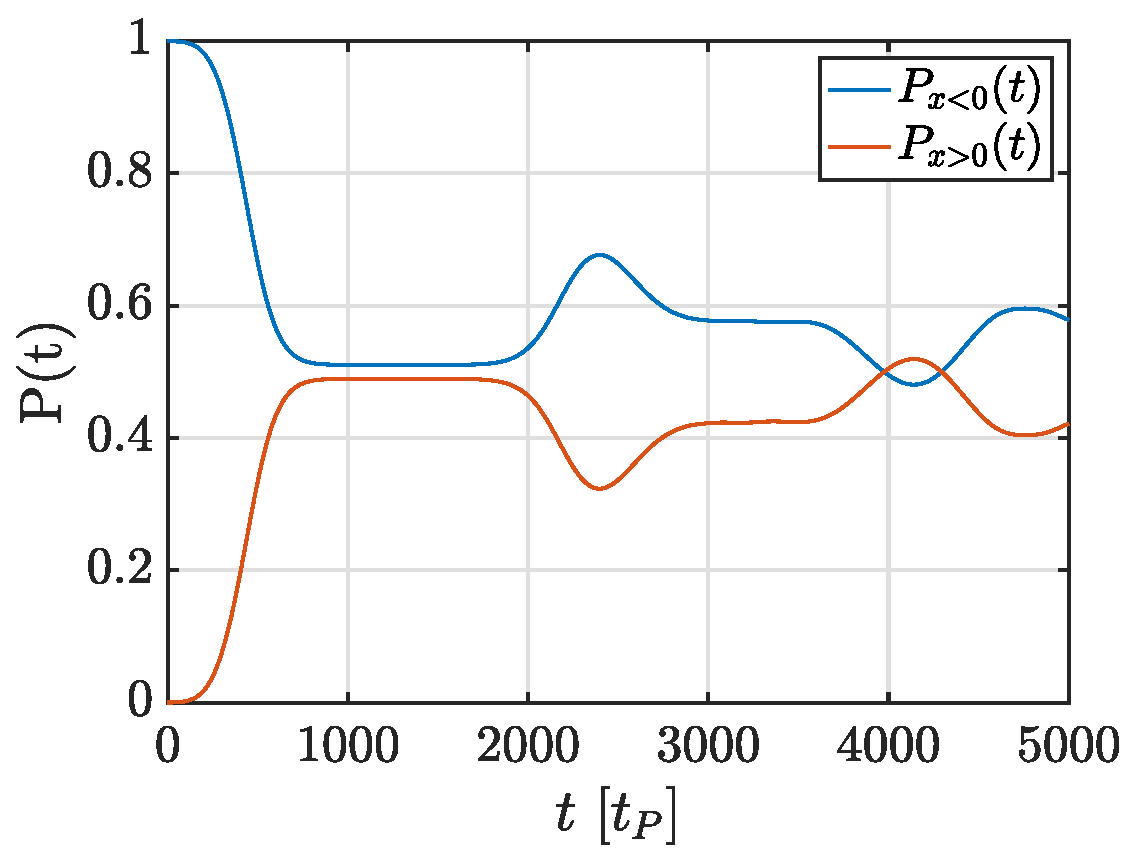
\includegraphics[width=\textwidth]{graphs/iii_findn_prob.eps}
          \caption{$P(t)$ with respect to t}
          \label{fig:iii_findn_prob}
        \end{subfigure}
        \caption{Evolution of the particle for $\Delta = \SI{64}{\Plength}$ and $\Delta t = \SI{5}{\Ptime}$ with $n=11$}
        \label{fig:iii_findn}
      \end{figure}


    \subsubsection{$n$ as real value}
      This time, $n$ is considered as real.
      The same process is applied that the previous section.
      Note that interpolating the result from the best values as a parabola does not make sense, as figure \ref{fig:iii_findn_cont_n} shows that the curve is straight.\\

      Figure \ref{fig:iii_findn_cont_n} gives the difference of probabilities with respect to $n$.
      The best value of $n$ is given by $n=\num{11.06}$ with a difference of probabilities at $t=\SI{1000}{\Ptime}$ given by $\abs{P_{x<0} - P_{x>0}} \approx \SI{5.13e-3}{\percent}$, which is much better than the integer result.\\

      \begin{figure}[h]
        \centering
        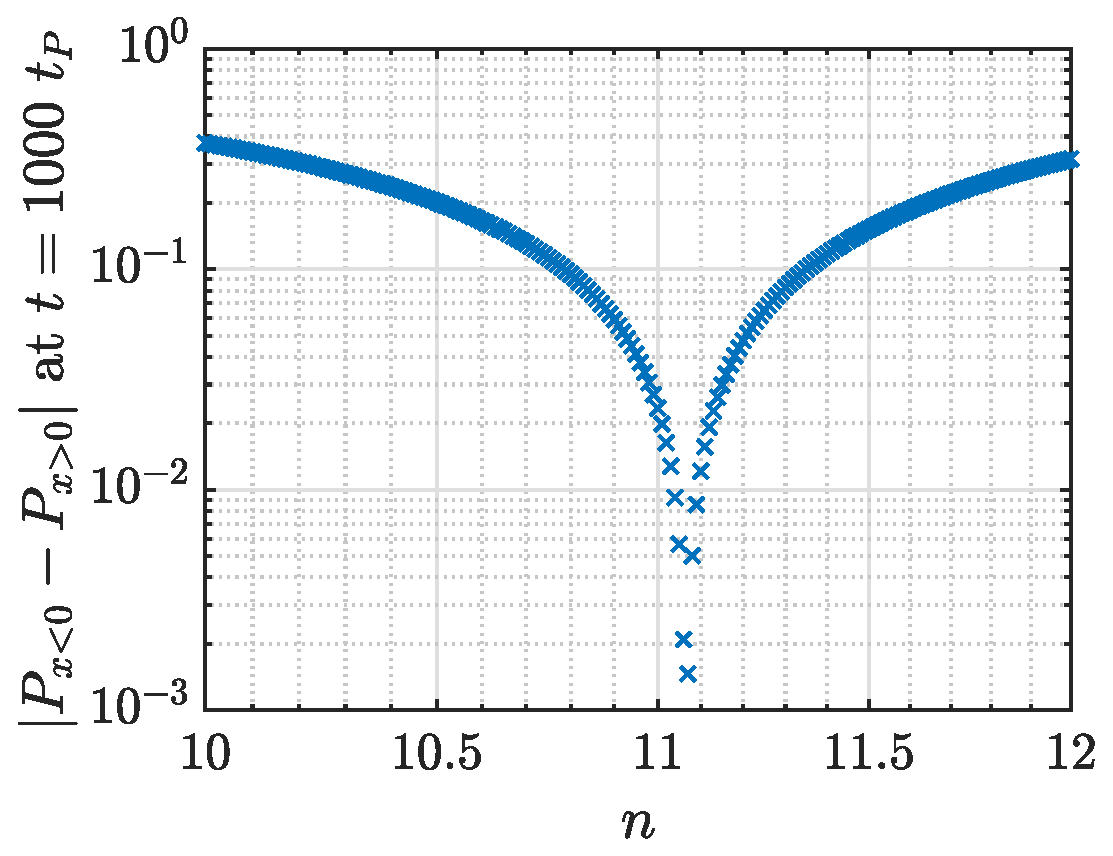
\includegraphics[width=0.45\textwidth]{graphs/iii_findn_cont_n.eps}
        \caption{Difference of probabilities for $\Delta = \SI{64}{\Plength}$ and $\Delta t = \SI{5}{\Ptime}$ with respect to real n}
        \label{fig:iii_findn_cont_n}
      \end{figure}

      The evolution of the system is given by figure \ref{fig:iii_findn_cont} with figure \ref{fig:iii_findn_cont_evo}, the evolution of the density of probability $\abs{\psi(x,t)}^2$ with respect to space and time, giving again a clear separation between both sides, and figure \ref{fig:iii_findn_cont_prob}, the evolution of both probabilities, giving an overlapping result for $t=\SI{1000}{\Ptime}$.\\

      \begin{figure}[h]
        \centering
        \begin{subfigure}[t]{0.45\textwidth}
          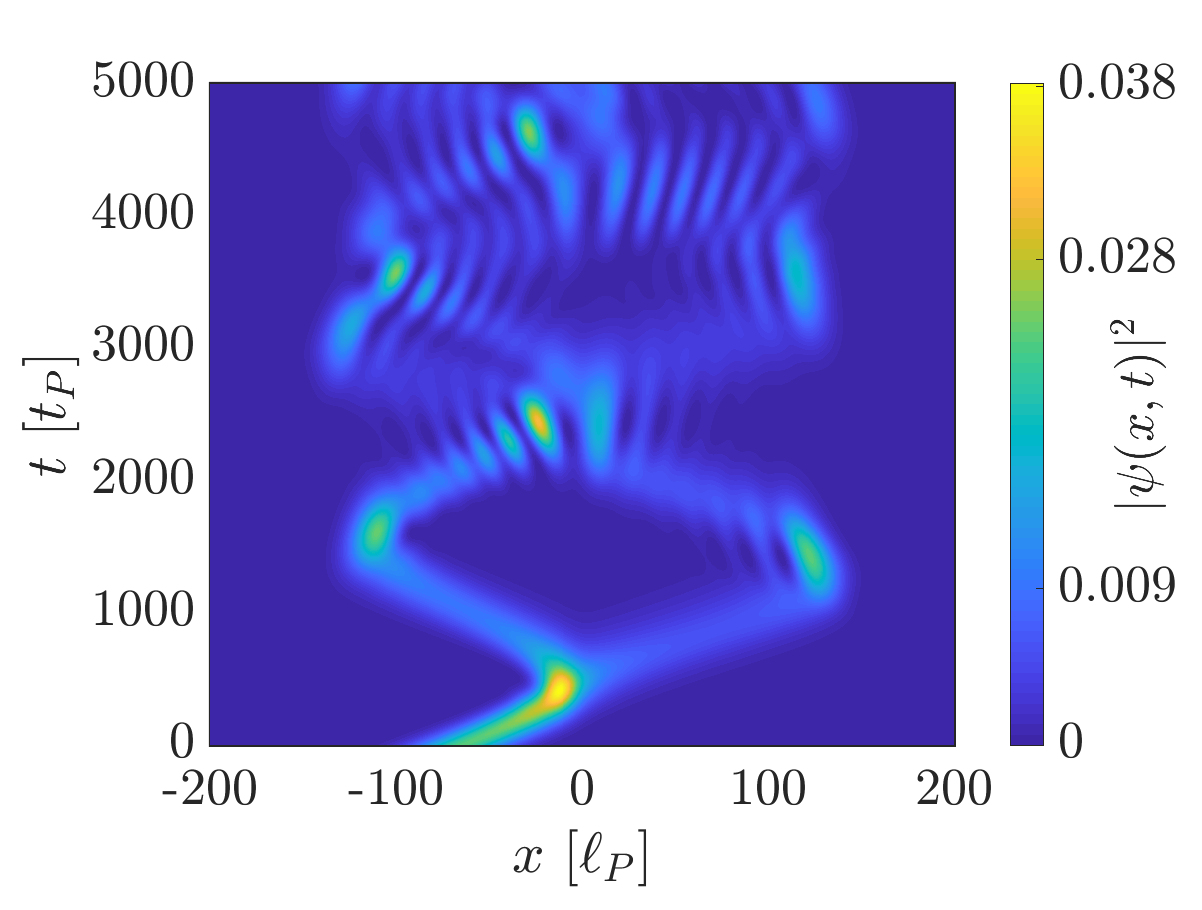
\includegraphics[width=\textwidth]{graphs/iii_findn_cont_evo.eps}
          \caption{$|\psi(x, t)|^2$ with respect to $x$ and $t$}
          \label{fig:iii_findn_cont_evo}
        \end{subfigure}
        ~
        \begin{subfigure}[t]{0.45\textwidth}
          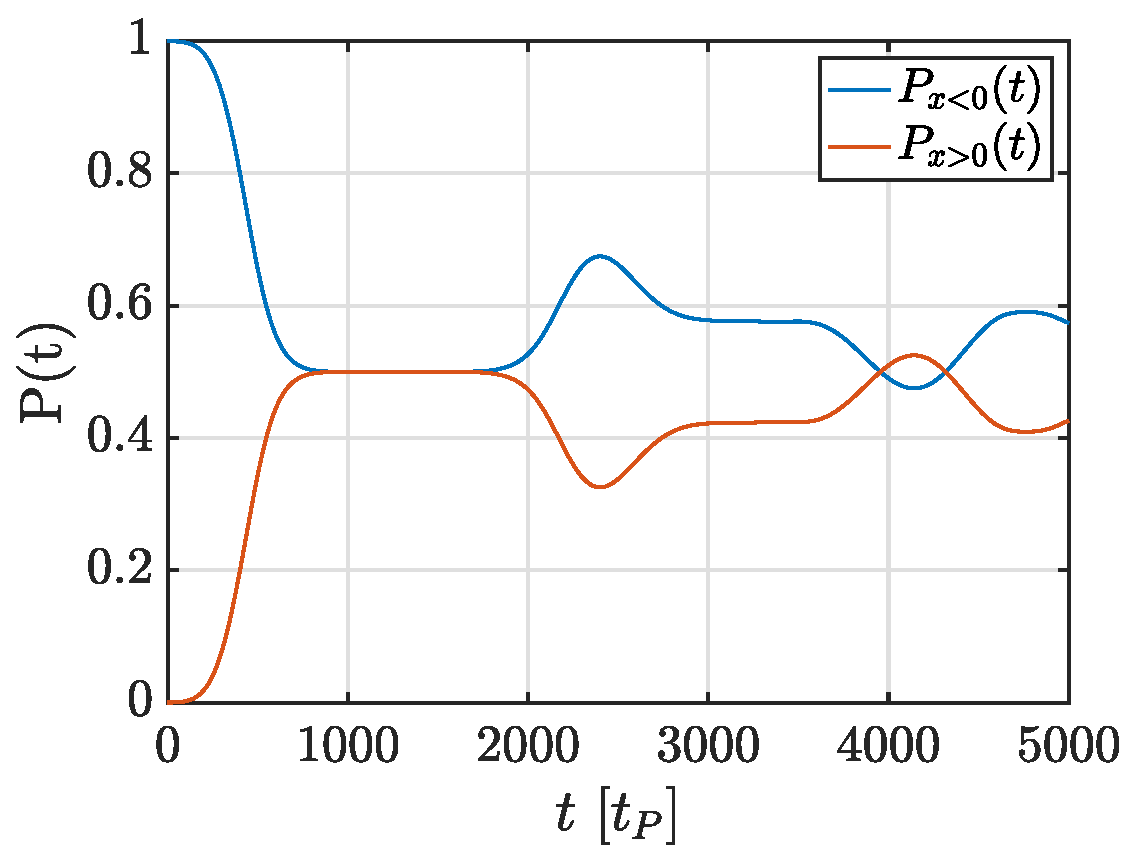
\includegraphics[width=\textwidth]{graphs/iii_findn_cont_prob.eps}
          \caption{$P(t)$ with respect to $t$}
          \label{fig:iii_findn_cont_prob}
        \end{subfigure}
        \caption{Evolution of the particle for $\Delta = \SI{64}{\Plength}$ and $\Delta t = \SI{5}{\Ptime}$ with $n=\num{11.06}$}
        \label{fig:iii_findn_cont}
      \end{figure}

      This way, a good $n$ to find a tunnelling probability of \SI{50}{\percent} has been found.

%%%%%%%%%%%%%%%%%%%%%%%%%%%%%%%%%%%%%%%%%%%%%%%%%%

\newpage
\section{Detection of a particle}

%%%%%%%%%%%%%%%%%%%%%%%%%%%%%%%%%%%%%%%%%%%%%%%%%%

\newpage
\section{Bonus}
  This section will present some additionnal studies to the report.\\

  \subsection{Alternative potential energy}
    This section presents the evolution of the system given by the following parameters, using some alternative definitions for the potential energy.
    The parameters are given by $x_L=\SI{-200}{\Plength}$, $x_R=\SI{200}{\Plength}$, $\omega = \SI{0.003}{\Pangularfrequency}$, $\Delta = \SI{64}{\Plength}$, $x_0 = -\Delta$, $\sigma_\text{norm} = \SI{0.06}{\Plength}$, $n=14$, $t_\text{fin} = \SI{5000}{\Ptime}$, $N_\text{inters} = 300$ and $\Delta t = \SI{2}{\Ptime}$, unless stated later.\\
    %TODO : Le "unless stated later" me semble moche. T'as une meilleure traduction pour "sauf future contre-indication" ?

      \subsubsection{Embed wave with a centered barrier}
        The potential is given by equation \eqref{eq:pot_A_pot}, represented as figure \ref{fig:v_pot_A_pot}.
        Note that numerically, $+\infty$ is simply given by a sufficiently high number.
        All values are expressed as Plank energy.

        \begin{equation}
          V(x) =
          \begin{cases}
            0.025,~\text{if $|x| \leq 5$}\\
            0,~\text{if $5 < |x| < 200$}\\
            +\infty,~\text{if $|x| < 200$}
          \end{cases}
          \label{eq:pot_A_pot}
        \end{equation}

        As $E<\max\bracket{V}$, figure \ref{fig:v_pot_A_evo} shows the effect of quantum tunnelling, as the particle has a probability of being on the right side.

        \begin{figure}[h]
          \centering
          \begin{subfigure}[t]{0.45\textwidth}
            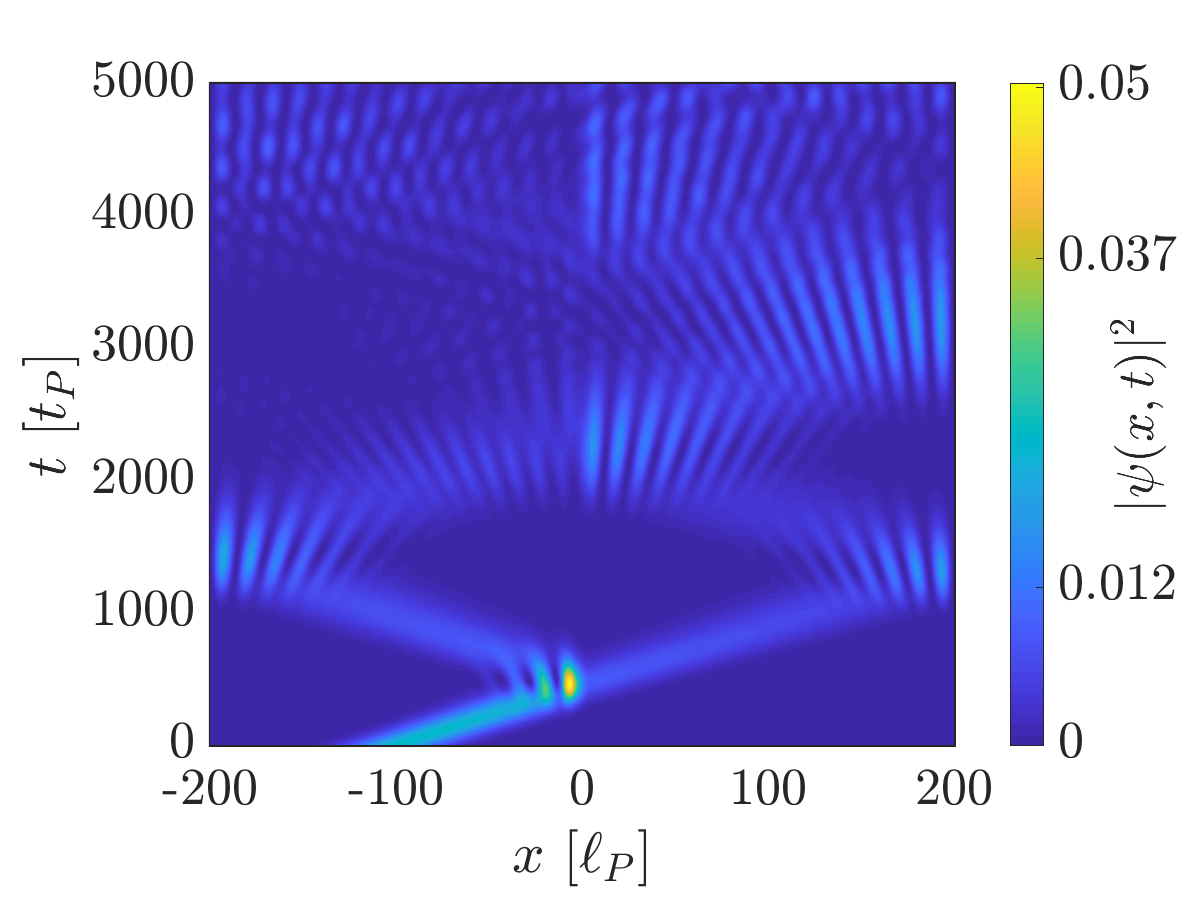
\includegraphics[width=\textwidth]{graphs/v_pot_A_evo.eps}
            \caption{$|\psi(x, t)|^2$ with respect to $x$ and $t$}
            \label{fig:v_pot_A_evo}
          \end{subfigure}
          ~
          \begin{subfigure}[t]{0.45\textwidth}
            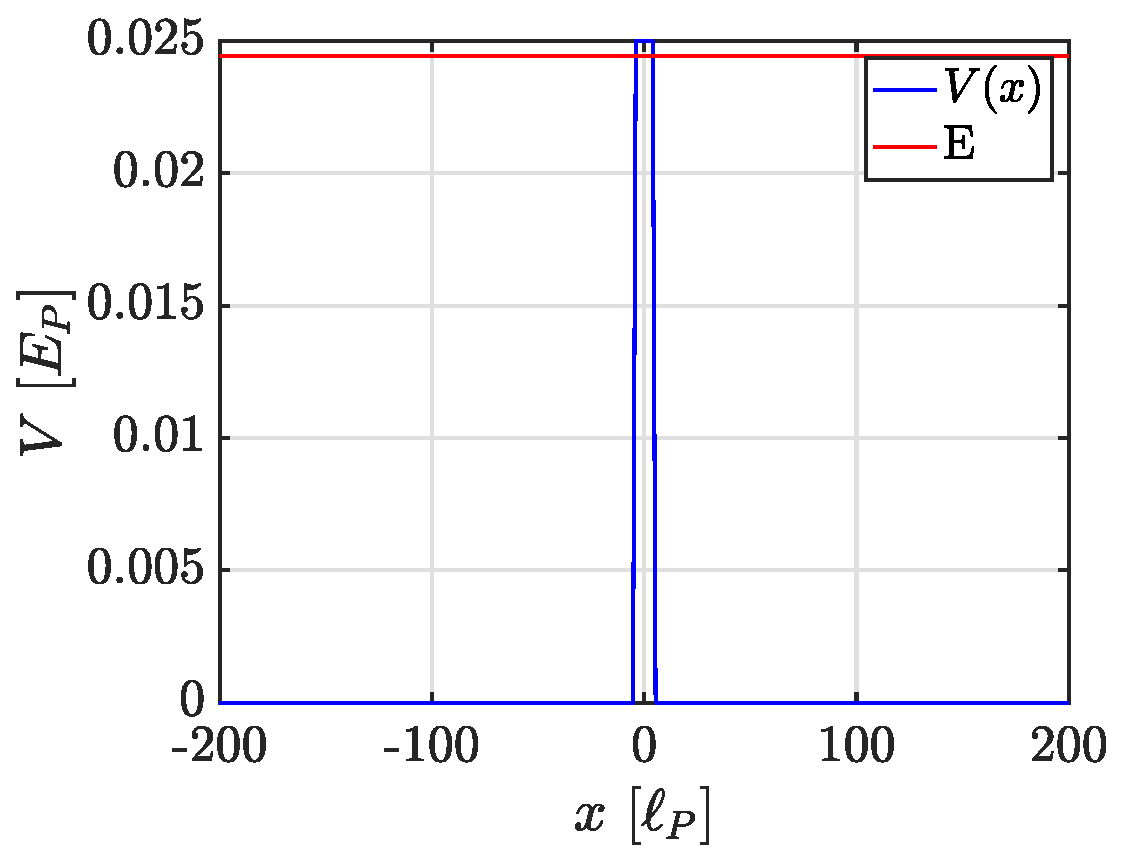
\includegraphics[width=\textwidth]{graphs/v_pot_A_pot.eps}
            \caption{potential energy $V$ with respect to $x$}
            \label{fig:v_pot_A_pot}
          \end{subfigure}
          \caption{Evolution of the system for the potential energy given by equation \eqref{eq:pot_A_pot}}
          \label{fig:v_pot_A}
        \end{figure}

      \subsubsection{Quantum tunnelling with respect to the width of the barrier}
        This additionnal study focuses on the transmission probability when the width of the potential barrier from equation \eqref{eq:pot_A_pot} changes.
        The potential energy is given by equation \eqref{eq:pot_conv}.
        All values are expressed as Plank energy.

        \begin{equation}
          V(x) =
          \begin{cases}
            0.1,~\text{if $|x| \leq \Delta$}\\
            0,~\text{if $\Delta < |x| < 200$}\\
            +\infty,~\text{if $|x| < 200$}
          \end{cases}
          \label{eq:pot_conv}
        \end{equation}

        In this section, $\Delta$ represents half of the width of the potential barrier and will vary as $\Delta \in \left[0, 6\right] \si{\Plength}$ with steps of \SI{0.3}{\Plength}.
        To get a good enough spacial definition allowing these steps, $N_\text{inters} = \num{5000}$ and to strongly reduce the computation time, $\Delta t = \SI{5}{\Ptime}$.
        All the points are taken at $t = \SI{1000}{\Ptime}$.

        Figure \ref{fig:v_conv_delta01} gives the probability for the particle to be on the right side at $t = \SI{1000}{\Ptime}$, which occures after the first quantum tunnelling.
        % This figure shows the non-linearity of this effect.
        % Lower widths give a concave curve, but at bigger widths, the curve becomes convex.
        % Thus, the quantum tunnelling slowly decreases and seems to tend to zero when the barrier has a bigger width.

        \begin{figure}[h]
          \centering
          \begin{subfigure}[t]{0.45\textwidth}
            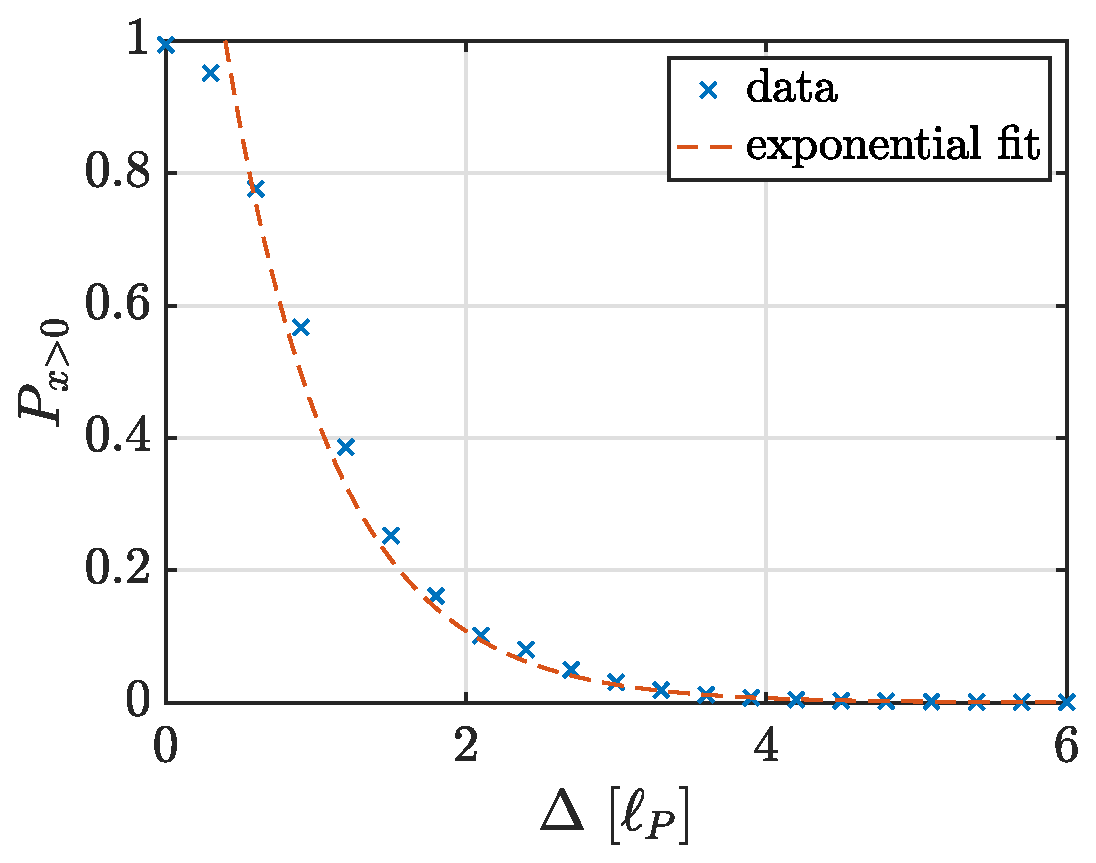
\includegraphics[width=\textwidth]{graphs/v_conv_delta01.eps}
            \caption{tut}
            \label{fig:v_conv_delta01}
          \end{subfigure}
          ~
          \begin{subfigure}[t]{0.45\textwidth}
            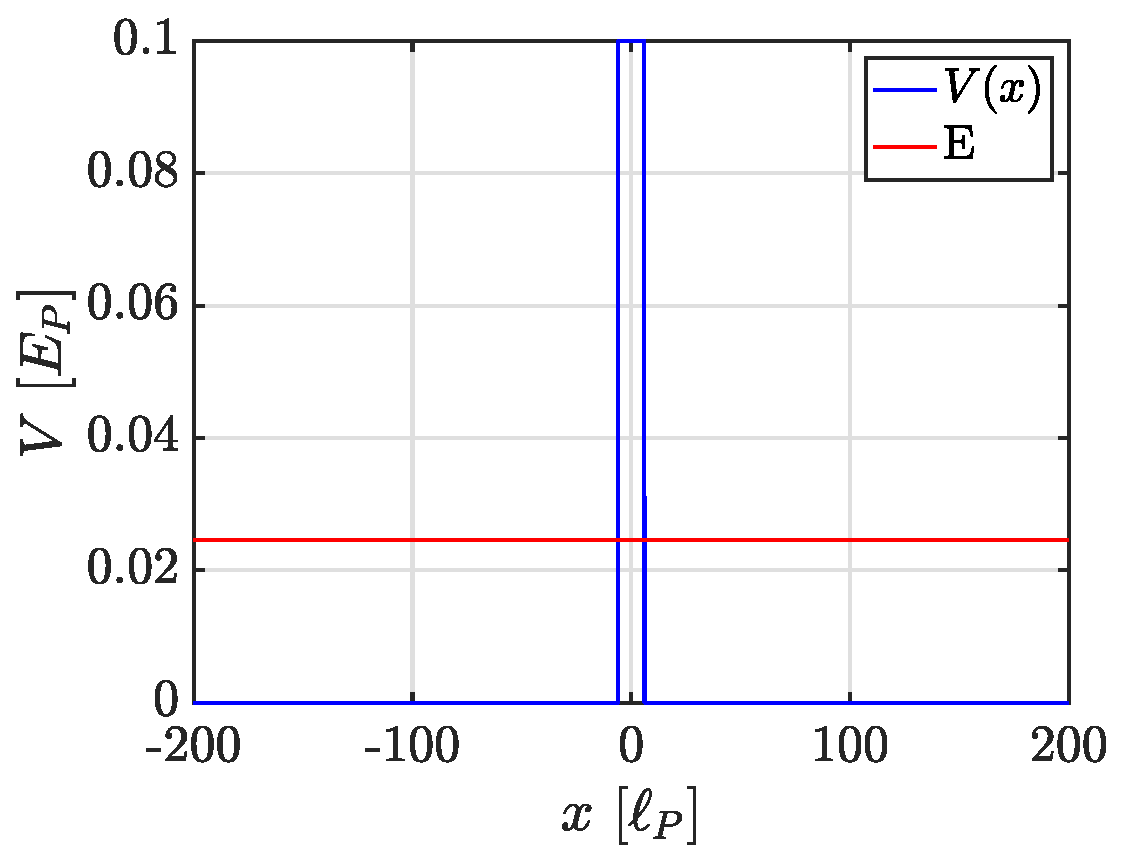
\includegraphics[width=\textwidth]{graphs/v_conv_delta_pot.eps}
            \caption{tut}
            \label{fig:v_conv_delta_pot}
          \end{subfigure}
          \caption{tut}
          \label{fig:v_conv_delta}
        \end{figure}

        % \begin{figure}[h]
        %   \centering
        %   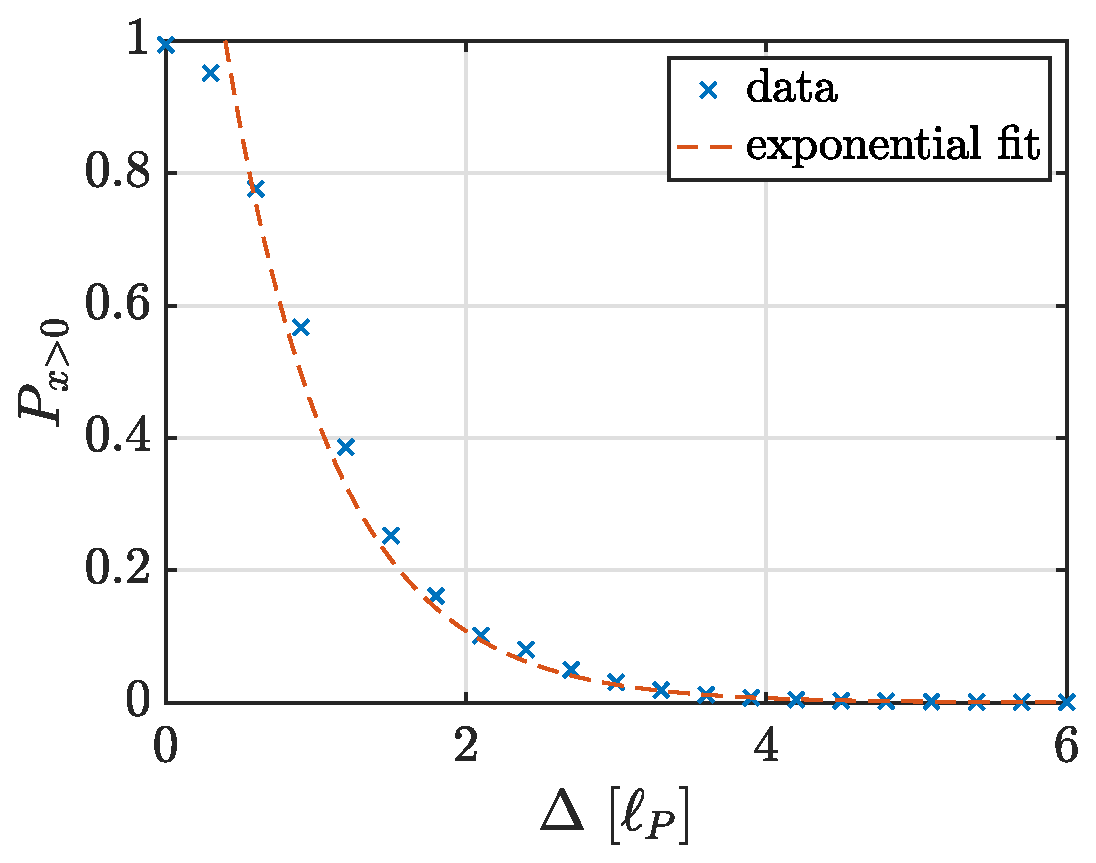
\includegraphics[width=0.45\textwidth]{graphs/v_conv_delta01.eps}
        %   \caption{Study of the left-side probability $P_{x>0}$ with respect to half of the potential barrier width $\Delta$ at $t=\SI{1000}{\Ptime}$}
        %   \label{fig:v_conv_delta}
        % \end{figure}

        As a summary, quantum tunnelling is a non-neglectable effect when the barrier to overcome is thinner but becomes neglectable when it gets thicker.

      \subsubsection{Periodic potential}
      This time, the potential energy, which is given by equation \eqref{eq:pot_Ba_pot}, is given as periodic.
      All values are expressed as Plank energy and again, $E<\max\bracket{V}$ as shown by the representation of the energy in figure \ref{fig:v_pot_Ba_pot}.

      \begin{equation}
        V(x) = 0.09\abs{\sin\bracket{\frac{x}{10}}}
        \label{eq:pot_Ba_pot}
      \end{equation}

      Figure \ref{fig:v_pot_Ba_evo} shows the evolution of the system and shows again the effect of quantum tunnelling.
      The particles as a probability to overcome the barriers multiple times, with a decreasing probability density the further from the origin.
      This figure also shows the global oscillation caused by the reflexion at the borders of the system.

      \begin{figure}[h]
        \centering
        \begin{subfigure}[t]{0.45\textwidth}
          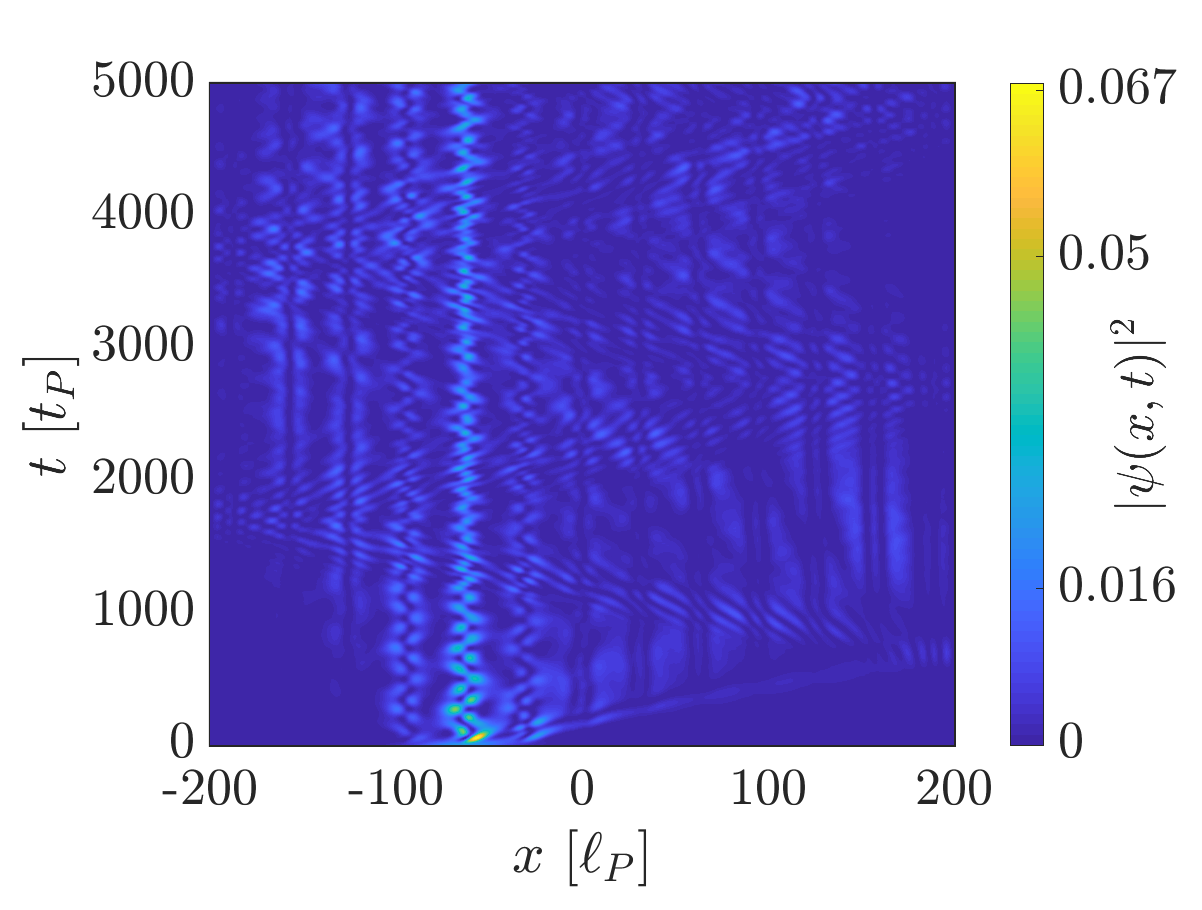
\includegraphics[width=\textwidth]{graphs/v_pot_Ba_evo.eps}
          \caption{$|\psi(x, t)|^2$ with respect to $x$ and $t$}
          \label{fig:v_pot_Ba_evo}
        \end{subfigure}
        ~
        \begin{subfigure}[t]{0.45\textwidth}
          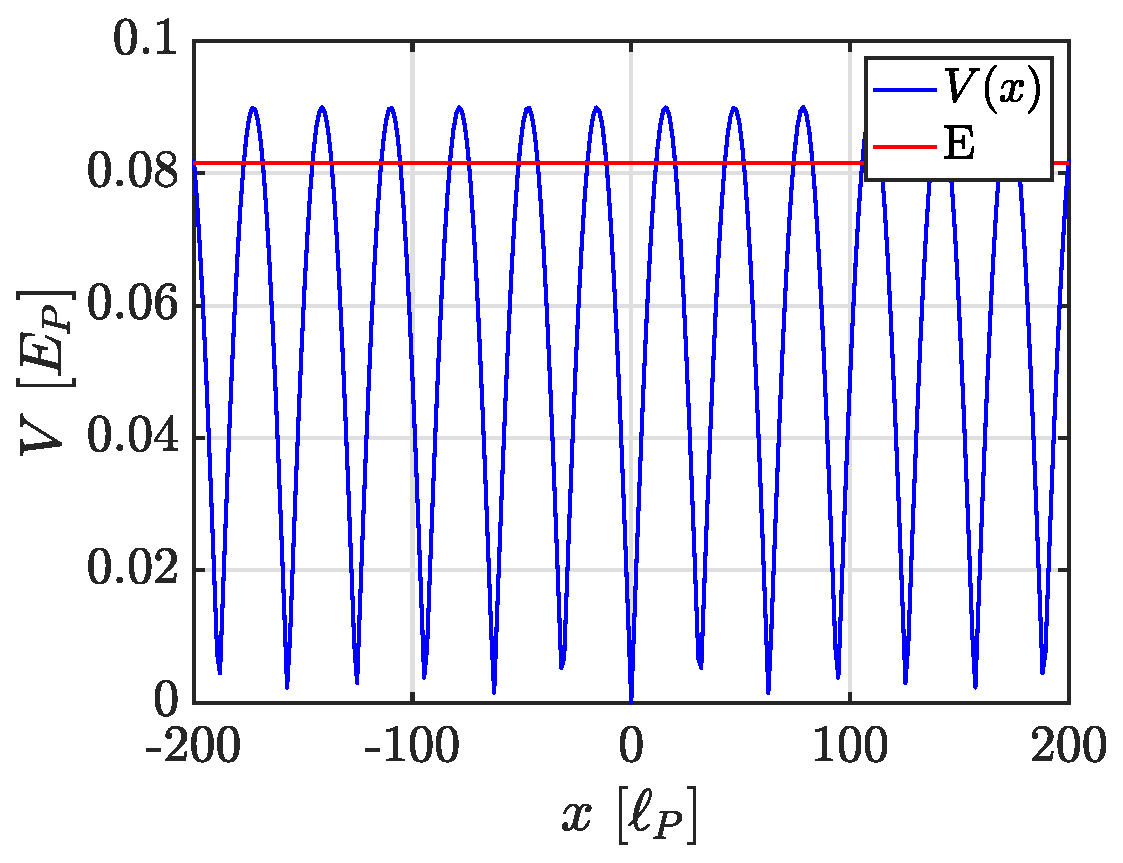
\includegraphics[width=\textwidth]{graphs/v_pot_Ba_pot.eps}
          \caption{potential energy $V$ with respect to $x$}
          \label{fig:v_pot_Ba_pot}
        \end{subfigure}
        \caption{Evolution of the system for the potential energy given by equation \eqref{eq:pot_Ba_pot}}
        \label{fig:v_pot_Ba}
      \end{figure}

    % \subsubsection{\textit{The light beacon}}
    %   The potential is given by equation \eqref{eq:pot_Bb_pot}, represented as figure \ref{fig:v_pot_Bb_pot}.
    %
    %   \begin{equation}
    %     V(x) = \abs{\sin\bracket{\frac{x}{100}}}
    %     \label{eq:pot_Bb_pot}
    %   \end{equation}
    %
    %   Figure \ref{fig:v_pot_Bb_evo} shows the evolution of the system with this potential.
    %   It is not a really significant example, but the plot of evolution (Fig. \ref{fig:v_pot_Bb_evo}) shows some density of probability suddenly stopping.
    %
    %   \begin{figure}[h]
    %     \centering
    %     \begin{subfigure}[t]{0.45\textwidth}
    %       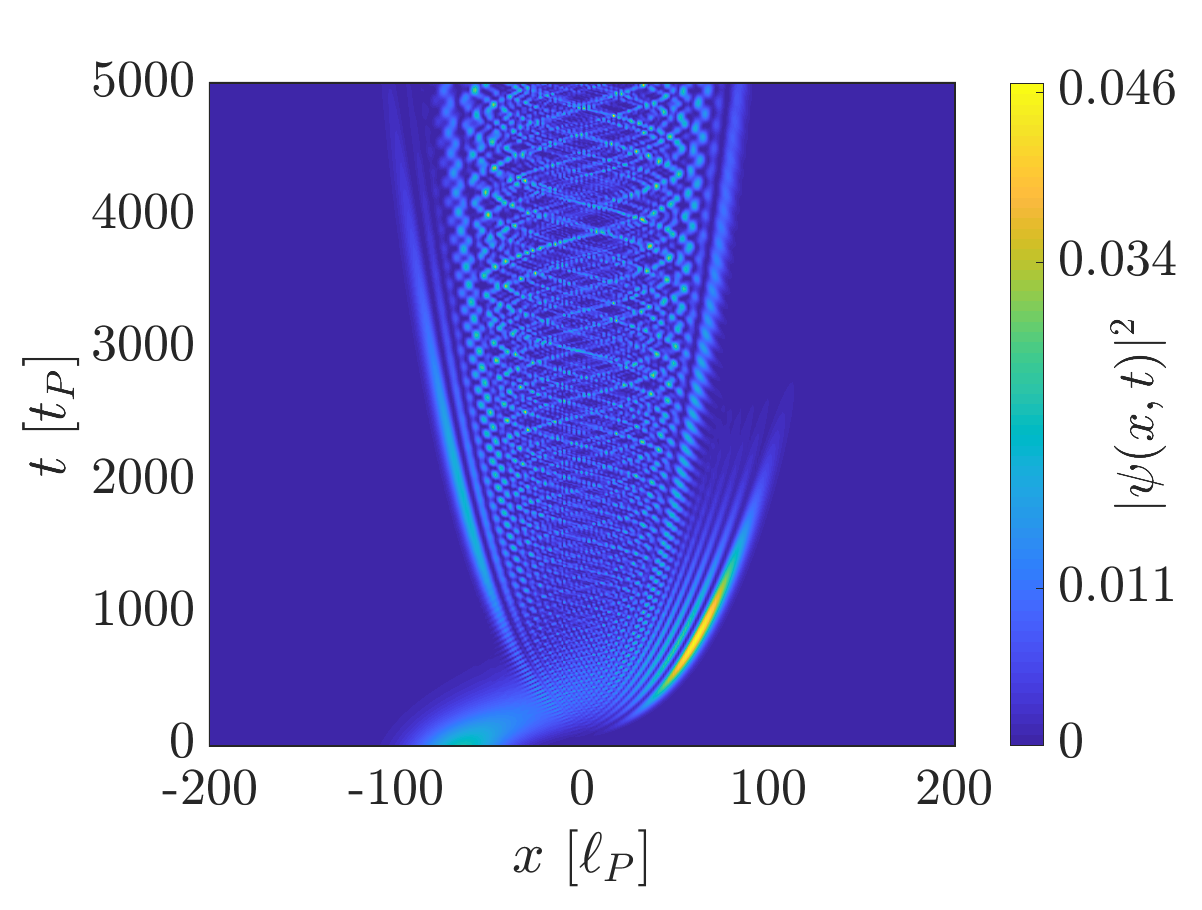
\includegraphics[width=\textwidth]{graphs/v_pot_Bb_evo.eps}
    %       \caption{$|\psi(x, t)|^2$ with respect to $x$ and $t$}
    %       \label{fig:v_pot_Bb_evo}
    %     \end{subfigure}
    %     ~
    %     \begin{subfigure}[t]{0.45\textwidth}
    %       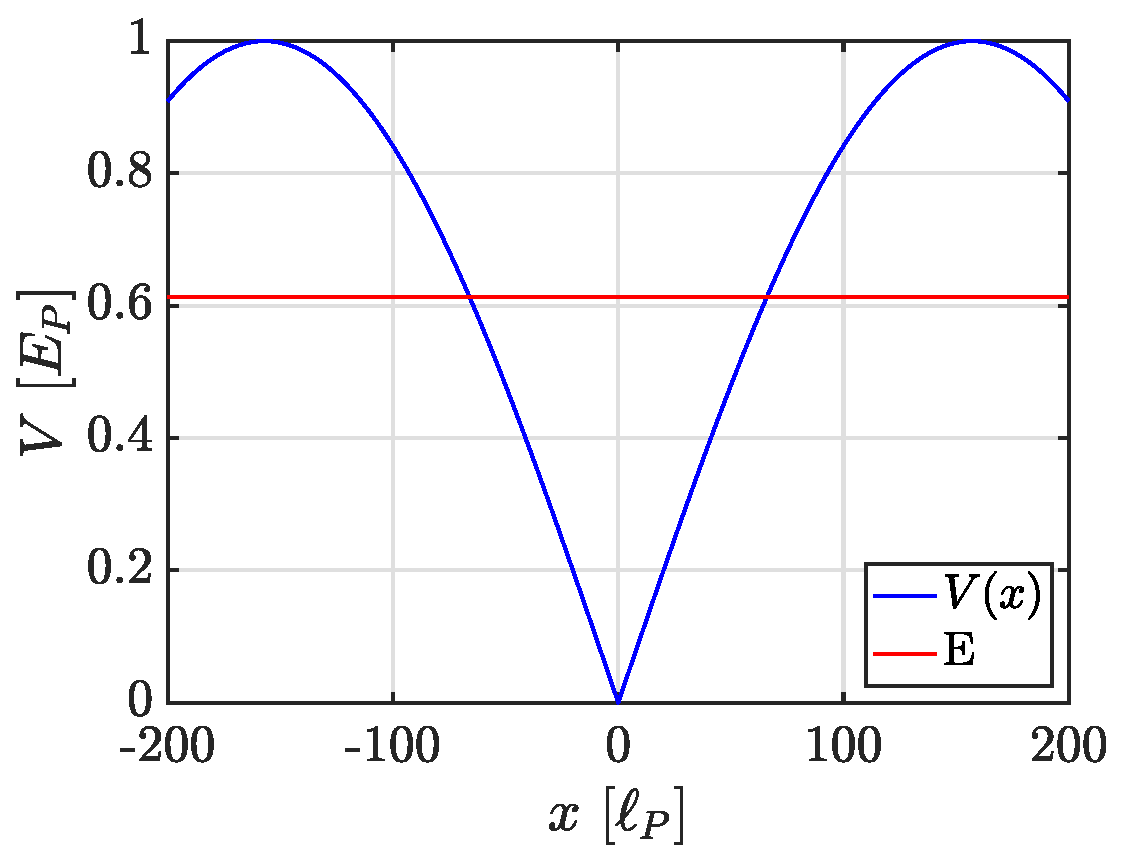
\includegraphics[width=\textwidth]{graphs/v_pot_Bb_pot.eps}
    %       \caption{potential energy $V$ with respect to $x$}
    %       \label{fig:v_pot_Bb_pot}
    %     \end{subfigure}
    %     \caption{Evolution of the system for the potential energy given by equation \eqref{eq:pot_Bb_pot}}
    %     \label{fig:v_pot_Bb}
    %   \end{figure}




\newpage
\begin{thebibliography}{99}
  \bibitem{wiki:quantum_tunnelling} Wikipedia contributors. (2019, May 6). Quantum tunnelling. In Wikipedia, The Free Encyclopedia. Retrieved 17:01, May 18, 2019, from \url{https://en.wikipedia.org/w/index.php?title=Quantum_tunnelling&oldid=895805434}
\end{thebibliography}

\end{document}
